\documentclass[11pt]{article}
\ifdefined\pdfinfoomitdate\pdfinfoomitdate=1\pdftrailerid{}\pdfsuppressptexinfo=15\fi
\usepackage[a4paper,margin=27mm]{geometry}
\usepackage[T1]{fontenc}
\usepackage{amsmath,amssymb,amsthm,booktabs,array,graphicx}
\usepackage[hidelinks]{hyperref}
\hypersetup{pdfauthor={Adam Buran},pdftitle={Last fall degrees of elliptic curve summation systems: machine-checked bounds and exact values}}
\newtheorem{theorem}{Theorem}
\newtheorem{lemma}[theorem]{Lemma}
\newtheorem{corollary}[theorem]{Corollary}
\newtheorem{proposition}[theorem]{Proposition}
\theoremstyle{remark}\newtheorem{remark}[theorem]{Remark}
\newcommand{\F}{\mathbb F}
\newcommand{\lfd}{\operatorname{LFD}}
\newcommand{\NF}{\operatorname{NF}}
\newcommand{\wt}{\operatorname{wt}}
\newcommand{\DEPTHTENMORE}{%
Two further instances give the same degree-$5$ closure. The second is a
proper ideal on the same curve family, $p=13313$, $y^2=x^3+x$, target
abscissa $7412$, with $98$ scalar solutions; the third is a random curve,
$p=15361$, $y^2=x^3+4021x+9917$, target abscissa $7776$, with $60$
solutions. In both the verified-closed $V_5$ has rank $18{,}569$ (targets
$21{,}602$ and $21{,}640$), does not contain $1$, and so $\lfd\ge6$. All three instances
have $\dim V_4=1549$ and the same symmetric and antisymmetric ranks
$9311+9258$ of $V_5$ under the summand swap.

\paragraph{The exact value at depth ten.}
For the unit instance the degree-$6$ closure contains $1$, so $\lfd=6$
exactly. The computation starts from the verified $V_5$ above, embeds it in the
degree-$6$ space, splits it into its parts symmetric and antisymmetric under
the summand swap $\sigma$ (both lie in $V_6$, since the system is
$\sigma$-invariant and $2$ is invertible), and adds, in each round, random
linear combinations of the $2k$ variable shifts of the rows whose leading
monomial has weight below $6$. Every added row is a product admitted by the
closure rule, so every row lies in $V_6$ whatever the random choices; the
certificate is one-sided and sound. After eight rounds both parts have full
rank, $30{,}318+30{,}142=60{,}460=|M_{\le6}|$, so $V_6=M_{\le6}\ni1$. The
falls are visible in the ranks: after round seven the rank is $59{,}371$,
above the $18{,}569+\binom{20}{6}=57{,}329$ that a closure without a new
element of weight below $6$ can reach, and round eight shifts exactly
$18{,}569+2042$ low rows.
An independent engine, started from
the generator alone, reaches the same closure in $453$ rounds: $V_6=M_{\le6}$
with part ranks $30{,}318+30{,}142$, $1\in V_6$, and a deterministic sweep of
all $21{,}700$ low rows with no residual. With the lower bound this gives the exact profile
$4$ for $k=2,\ldots,5$, $5$ for $k=6,\ldots,9$ and $6$ at $k=10$ on the
instances computed, matching the averaged degree of regularity that Petit,
Kosters and Messeng report for the same subgroup-chain presentation at every depth $k=2,\ldots,10$, and at $k=11$~\cite[Table~4]{pkm}.

\paragraph{Depths eleven to fourteen.}
Two sets of closures extend the depth-ten measurement: closures of an
independent engine at depths $11$ to $13$ over $p=12289$ and $p=40961$, and
closures of a third engine on a GPU at depths $10$ to $16$ over $p=65537$
and at depths $13$ and $14$ over $p=114689$ and $p=163841$.
The independent engine (written without reference to the other engines of
this paper, with a full deterministic closure sweep)
reproduces $\dim V_5=18{,}569$ on all three depth-ten instances and computes
$\dim V_5=25{,}033$ at $k=11$ on two instances ($p=12289$, a unit ideal on
$y^2=x^3+x$ and a proper ideal with $348$ solutions on
$y^2=x^3+4021x+9917$), closed and without $1$. Since $|Z|\le2^{k+1}$, the
degree-$5$ part of the ideal has dimension at least
$\binom{22}{\le5}-4096=31{,}347>25{,}033$, so $\lfd\ge6$ at $k=11$ for both. The same engine gives
$\dim V_4=4k^2+172k-571$ on two instances at every $k=6,\ldots,13$.
At $k=12$ the same engine gives $\dim V_5=32{,}057$ on both instances
($p=12289$; $y^2=x^3+x$ with $1352$ solutions and $y^2=x^3+4021x+9917$ with
$1399$), with identical profile $(0,0,2,146,3727,32057)$ and part ranks
$16{,}061+15{,}996$, and at $k=13$ ($p=40961$, the same two curves, $1484$
and $1582$ solutions) $\dim V_5=39{,}657$ on both, profile
$(0,0,2,150,4021,39657)$, part ranks $19{,}864+19{,}793$; every closure is
closed by a deterministic sweep of all its low rows ($3727$, resp.\ $4021$).
Since $\binom{24}{\le5}-2^{13}=47{,}263>32{,}057$ and
$\binom{26}{\le5}-2^{14}=67{,}298>39{,}657$, $\lfd\ge6$ at $k=12$ and
$k=13$ as well.

\paragraph{A unit instance over $p=65537$.}
Let $p=65537=2^{16}+1$, $E:y^2=x^3+x$ and $R=(4271,11720)\in E(\F_p)$. The
same $(a,b,R)$ is used at every depth. The point of this instance is that
its ideal is the unit ideal at every depth $k\le15$, by the following lemma.

\begin{lemma}[A unit instance at depths up to fifteen; written]\label{lem:unit}
Let $X=4271$ and let $H\subset\F_p^*$ be the subgroup of order $2^k$ with
$2\le k\le15$. There is no pair $(x_1,x_2)\in H^2$ with $S_3(x_1,x_2,X)=0$.
Hence the two-summand chain system of $E$ with target abscissa $X$ has no
scalar solution, and its ideal is the unit ideal, at every such depth.
\end{lemma}
\begin{proof}
One checks $X^{(p-1)/2}=-1$, so $X$ is not a square in $\F_p$, and
$X^3+X=Y^2$ with $Y=11720$. The group $\F_p^*$ is cyclic of order $2^{16}$
and its squares form the subgroup of order $2^{15}$, so $H$ consists of
squares for $k\le15$. The roots $\pm i$ of $x^2+1$ have order $4$, hence are
squares, so $X\notin\{0,\pm i\}$ and therefore $Y\ne0$.
Let $\alpha:E(\F_p)\to\F_p^*/\F_p^{*2}$ be given by $\alpha(O)=1$,
$\alpha((0,0))=1$ and $\alpha((x,y))=x$ otherwise. It is a group
homomorphism: it is the descent map of the $2$-isogeny with kernel
$\{O,(0,0)\}$ of a curve $y^2=x(x^2+ax+b)$, here with $b=1$
\cite[Prop.~X.4.9]{silv}, and its proof is algebraic and holds over every
field of characteristic different from two.

Suppose $S_3(x_1,x_2,X)=0$ with $x_1,x_2\in H$. By the defining property of
$S_3$ (which also covers $x_1=x_2$, where $S_3$ has degree at most one in the
last variable), there are points $P_1,P_2\in E(\overline{\F}_p)$ with
$x(P_i)=x_i$ and $x(Q)=X$ for $Q=P_1+P_2$, after replacing $P_2$ by $-P_2$ if
necessary. Both $P_i$ are affine and not $(0,0)$, since $x_i\in H$. Let
$\varphi$ be the $p$-power Frobenius. As $x_i\in\F_p$, $y(P_i)^2\in\F_p$, so
$\varphi P_i=\pm P_i$.
\begin{enumerate}
\item[(a)] $\varphi P_1=P_1$ and $\varphi P_2=P_2$. Then $Q\in E(\F_p)$ with
 $x(Q)=X$, so $Q=\pm R$ and $\alpha(Q)=\alpha(R)=X$. But
 $\alpha(Q)=\alpha(P_1)\alpha(P_2)=x_1x_2$ is a square. This contradicts
 that $X$ is not a square.
\item[(b)] $\varphi P_1=-P_1$ and $\varphi P_2=-P_2$. Then $\varphi Q=-Q$, so
 $y(Q)^p=-y(Q)$, and $y(Q)^2=X^3+X\ne0$ gives
 $(X^3+X)^{(p-1)/2}=y(Q)^{p-1}=-1$. But $X^3+X=Y^2$ with $Y\in\F_p^*$, so
 $(X^3+X)^{(p-1)/2}=Y^{p-1}=1$.
\item[(c)] Otherwise, after exchanging the points, $\varphi P_1=P_1\ne-P_1$ and
 $\varphi P_2=-P_2\ne P_2$ (a point with $P=-P$ has both signs and falls under
 (a) or (b) according to the other point). Then $\varphi Q=P_1-P_2$, and
 $x(\varphi Q)=\varphi(X)=X=x(Q)$ gives $P_1-P_2=\pm(P_1+P_2)$, so $2P_2=O$ or
 $2P_1=O$, a contradiction.
\end{enumerate}
So the scalar solution set $Z$ is empty. The chain ideal is radical with all
points rational, so the full ideal is the vanishing ideal of $Z$, the unit
ideal.
\end{proof}
A direct enumeration of $Z$ at $k=10,\ldots,14$ also finds no point. The
lemma is not formalized.

\paragraph{A third engine.}
The runs below use a third implementation of the closure, written
separately from the other two and run on a GPU. It computes the reduced row
echelon basis of $V_D$ for the fixed column order (weight descending) of
the independent engine above, which we call the reference engine. This
basis depends only on the subspace, so equal basis hashes of two engines test
the whole computation. The engine was validated by equality of both basis
hashes with the reference engine on all cases small enough to run on a
workstation (eighteen closures at
$k=6,7$ and $D=3,4,5$ in four execution modes, the degree-$5$ closures at
$k=9,10$, ten cases over $p=65537$ at $k=6,7,8$, interrupted and resumed
runs), by a negative control in which the shifts of one row are withheld
(every withholding that changed the result was caught by the sweep), and by a self-test on the GPU that compares CPU,
GPU and the reference engine on eight cases. Every run below ends with a deterministic full sweep: every
shift of every final low row, in both swap parts, reduces to zero against the
final basis, with zero repairs. A space that passes the sweep is closed and
contains the generator, so it contains $V_D$, and every row added by the
engine is a reduction residual of a shift of an earlier row, so it lies in
$V_D$; rank, profile and membership of $1$ are therefore statements about
$V_D$ itself. The system generator ($S_3$ coefficients, chain normal form,
enumeration of $Z$) is shared with the reference engine and cross-checked
against one further implementation; it is not re-derived independently. The
$k=14$, $D=6$ runs used a variant that moves part of the basis to host
memory; it passed the same self-test.

In the other direction, the reference engine reproduces both basis hashes
of the GPU engine for $V_5(14)$ on the unit instance below ($122{,}438$
columns, dimension $47{,}849$) and confirms $V_6(10)=M_{\le6}$ and
$V_6(11)=M_{\le6}$, so the largest
degree-$5$ closure of that instance is computed by two engines with the same
canonical basis. The $k=14$, $D=6$ closure of the instance was run twice,
with different settings, and both runs give the same two basis hashes. An
independent checker, a separate program that shares no code with the
engines, read the stored basis $W$ of the
second run and verified the containing-space certificate directly: the basis
is in reduced echelon form, the generator lies in $W$, each of the $28$
shifts of each of the $73{,}587$ low rows reduces to zero against $W$ in
both swap parts ($4{,}120{,}872$ checks, no failure), and $1\notin W$. Its
rank, profile and basis hashes equal the engine's. The description of the
checker in the repository states which parts of the engine its author had
read.

\paragraph{Results to depth fourteen.}
All values in this paragraph are exact. On the unit instance the degree-$5$ closure is
closed and misses $1$ at $k=10,\ldots,15$, with
$\dim V_5=18{,}569$, $25{,}033$, $32{,}057$, $39{,}657$, $47{,}849$,
$56{,}649$ and profiles
\begin{gather*}
(0,0,2,138,3163,18569),\quad(0,0,2,142,3441,25033),\quad(0,0,2,146,3727,32057),\\
(0,0,2,150,4021,39657),\quad(0,0,2,154,4323,47849),\quad(0,0,2,158,4633,56649);
\end{gather*}
for $k\le13$ these are the dimensions and
profiles of the independent engine on the earlier instances. The degree-$6$
closure is the whole degree-$6$ space and contains $1$ at $k=10,11,12,13$
($\dim V_6=60{,}460$, $110{,}056$, $190{,}051$, $313{,}912$). With the
exclusion of $1$ from $V_5$, the last fall degree of this system is exactly
$6$ at $k=10,\ldots,13$. The upper side at $k=11,12,13$ is new. At $k=14$ the
degree-$6$ closure is closed and has dimension $448{,}922$ in the
$499{,}178$-dimensional space $M_{\le6}$ (codimension $50{,}256$), with low
profile $(0,0,2,154,4451,73587)$, and it does not contain $1$. Since $1$
lies in the ideal, $\lfd\ge7$ at $k=14$. By Theorem~\ref{thm:restrict}, $1\notin V_6(15)$
as well, and the ideal is the unit ideal at $k=15$ (Lemma~\ref{lem:unit}),
so $\lfd\ge7$ at $k=15$ on this instance too. The codimension of $V_D$ in
$M_{\le D}$ at the first deficient depth $4D-10$ is $10$, $189$, $3131$ and
$50{,}256$ for $D=3,4,5,6$.

\paragraph{The degree-seven step at depth fourteen.}
The space $M_{\le7}$ at $k=14$ has $1{,}683{,}218$ columns, too many for a
direct closure on the hardware we used. The exact value was obtained by a
degree lift, which computes $V_{D+1}$ from a closed $V_D$ without a closure
in $M_{\le D+1}$; the full statement, proof and algorithm are in the
repository (Section~\ref{sec:artifacts}). Call a
weight-$D$ monomial regular if its swap orbit is a pivot column of $V_D$ in
both swap parts, and a weight-$(D+1)$ monomial regular if all its
weight-$D$ divisors are. Modulo $V_D$, a shift of a basis row has at most
one regular coordinate of weight $D+1$. The regular top columns are
therefore eliminated by subtracting generators that share a column, and
what remains is a subspace $K$ of the small space $T$ spanned by the
non-regular top columns and the free columns of $V_D$. The elements of $K$
without top part are the falls. They are added to $V_D$ and shifted in
turn, until no new fall appears. At that fixed point
$V_{D+1}\cap M_{\le D}$ is $V_D$ plus the falls,
$\dim V_{D+1}=\dim V_D+\sum_q(r_q+\dim K_q)$ over the two swap parts $q$,
with $r_q$ the number of regular top columns of the part, and
$1\in V_{D+1}$ if and only if $1\in V_D$ or the class of $1$ is a fall. The
proof is written and not formalized.

On the unit instance the lift started from the checked basis of $V_6(14)$,
which has $25{,}136+25{,}120$ free columns. There are $1406$ non-regular
monomials of weight $6$; each part has $586{,}501$ regular and $5519$
non-regular columns of weight $7$, and $\dim T=30{,}655$ and $30{,}639$.
The lift reached its fixed point in three rounds, with $494+494$,
$12{,}260+12{,}260$ and $12{,}382+12{,}366$ new falls: every free column of
$V_6$ becomes a fall, $K=T$ in both parts, and
\[
 \dim V_7(14)=448{,}922+2\cdot586{,}501+30{,}655+30{,}639=1{,}683{,}218=|M_{\le7}|.
\]
So $V_7(14)$ is the whole space and contains $1$, and with $1\notin V_6(14)$
the last fall degree of this system is exactly $7$ at $k=14$ ($751$ seconds on the GPU). The coverage check
of the computation held: every regular weight-$7$
column was met in exactly one batch, with all seven of its generators.

The lift agrees with the direct closure in $170$ runs over $37$ cases with
$D\le5$ and $k\le11$, over the primes $12289$, $15361$, $65537$ and
$16777213$ (for the last, as polynomial systems, since $4\,\|\,p-1$): the dimension, the profile, the membership of $1$ and the
canonical hash of $V_{D+1}\cap M_{\le D}$ in both parts are equal in every
run. The cases include instances with solutions, where the lifted space
equals the ideal part, and the transitions at which $1$ enters, $D=4\to5$
at $k=6,\ldots,9$ and $D=5\to6$ at $k=10$; the last is the analogue of the
present step one degree lower, and the lift also reproduced it on the GPU.
Negative controls that withhold the iteration of the falls, or all shifts
of one index, change the result whenever the withheld rows are not
redundant. \LIFTCONTROL

A control at $k=14$ was then run on the random curve over $p=114689$
described below, which has $2370$ solutions. There the lifted space lies in
the ideal, so its dimension is at most $1{,}683{,}218-2370=1{,}680{,}848$,
and a lift that overshoots would be caught. From a kept, closed $V_6(14)$ of
that instance (dimension $448{,}922$, with the profile of the unit instance)
the lift reached its fixed point in three rounds, with $494+494$,
$12{,}260+12{,}260$ and $11{,}197+11{,}181$ new falls and $K$ of codimension
$1185$ in $T$ in each part. It gives $\dim V_7(14)=1{,}680{,}848$, exactly
the bound, without $1$, and $\dim(V_7\cap M_{\le6})=496{,}808=499{,}178-2370$.
The evaluation of $M_{<6}$, and hence of $M_{<7}$, on $Z$ has rank $2370$, computed directly with the degree-$6$ closure (\code{experiments/\allowbreak{}ic-bounds-k14/\allowbreak{}relaunch/\allowbreak{}fetched/\allowbreak{}proper-p114689-k14-D6.json}); the dimension count alone gives only the trivial bound $\le2370$. So $V_7$ is the degree-$7$
part of the ideal, and the local-to-global criterion gives $\lfd\le7$; since
$V_6$ is $47{,}886$ dimensions short of the degree-$6$ part of the ideal,
$\lfd=7$ exactly on this curve as well ($4679$ seconds; every regular
column covered once).

The lift was then run on the second unit instance, $y^2=x^3+3x$ over
$p=163841$ (below). A second run of its degree-$6$ closure, with the basis
kept, reproduced both basis hashes of the first run; the independent checker
passed on the kept basis; and the lift reached its fixed point in three
rounds with the same counts as over $p=65537$ ($K_\pm=T_\pm$, new elements
$494+494$, $12{,}260+12{,}260$, $12{,}382+12{,}366$): $V_7(14)=M_{\le7}$ and
$1\in V_7(14)$, so $\lfd=7$ exactly on this instance as well ($677$ seconds).

Unlike the closures above, the lift does not end with a sweep in
$M_{\le7}$ and produces no basis of $V_7$. The value $7$ therefore has no
independent certificate: it rests on the written proof, on the assertions
of the runs, on the comparisons just listed and on the control, and it is
one implementation, run once on each of three instances.

\paragraph{A random-curve replication.}
The same engine, on $y^2=x^3+4021x+9917$ over $p=65537$ (seed $12$, target
$(1424,826)$, $1028$ solutions at $k=13$ and $4068$ at $k=14$), gives the same
degree-$5$ dimensions and profiles, $39{,}657$ at $k=13$ and $47{,}849$ at
$k=14$, against $\dim(I\cap M_{\le5})=82{,}654$ and $118{,}370$. At $k=13$ the
degree-$6$ closure has dimension $312{,}884=313{,}912-1028$, equal to the
degree-$6$ part of the ideal, and the evaluation of $M_{<6}$ on $Z$ has rank
$1028$, so the local-to-global criterion gives $\lfd=6$ exactly on this
instance at $k=13$. At $k=14$ the degree-$6$ closure of this instance is
closed and has dimension $448{,}922$, with profile
$(0,0,2,154,4451,73587,448922)$ and part ranks $224{,}688+224{,}234$: the
same dimension, profile and part ranks as on the unit instance. The
degree-$6$ part of the ideal has dimension $499{,}178-4068=495{,}110$ (the
evaluation of $M_{\le6}$, and already of $M_{<6}$, on $Z$ has rank $4068$), so
$V_6$ misses it by $46{,}188$ dimensions and $\lfd\ge7$ at $k=14$ on the
random curve as well. As for $V_5$, the dimension of $V_6$ at these depths
does not depend on the instance.

\paragraph{Two more primes.}
The engine was also run over $p=163841=5\cdot2^{15}+1$ and
$p=114689=7\cdot2^{14}+1$. Over $p=163841$ the instance is $y^2=x^3+3x$
with target $(73730,28291)$. Its ideal is the unit ideal for $k\le14$: the
proof of Lemma~\ref{lem:unit} applies with $X=73730$, a non-residue with
$X^3+3X=28291^2\ne0$, because the subgroup of order $2^k$ lies in the
squares for $k\le14$; the enumeration of $Z$ at $k=13,14$ also gives no
point. At $k=13$, $\dim V_5=39{,}657$ without $1$ and $V_6=M_{\le6}\ni1$,
so $\lfd=6$ exactly. At $k=14$, $\dim V_5=47{,}849$ and $V_6$ is closed of
dimension $448{,}922$ without $1$, so $\lfd\ge7$. Profiles and part ranks
equal those over $p=65537$ at both depths.

Over $p=114689$ the instance is the random curve $y^2=x^3+31415x+92653$
with target $(80359,998)$ (seed $22$; $594$ solutions at $k=13$ and $2370$
at $k=14$). At $k=13$, $\dim V_5=39{,}657$, and $V_6$ is closed of dimension
$313{,}318=313{,}912-594$ with $\dim(V_6\cap M_{\le5})=83{,}088=83{,}682-594$.
The evaluation of $M_{<6}$ on $Z$ has rank $594$, computed directly (\code{experiments/\allowbreak{}ic-bounds-k14/\allowbreak{}runs/\allowbreak{}proper-p114689-k13-D6.json}); since $V_6$ lies in the ideal, $V_6$ equals the degree-$6$ part of the ideal; $V_5$ is $43{,}431$ dimensions short of the
degree-$5$ part. The local-to-global criterion gives $\lfd=6$ exactly, as on
the random curve over $p=65537$. At $k=14$, $\dim V_5=47{,}849$ with the same profile, and the degree-$6$
closure is closed of dimension $448{,}922$, with the profile and part ranks
of the other instances, against $496{,}808$ for the degree-$6$ part of the
ideal, so $\lfd\ge7$; the control lift above gives $\lfd=7$. The
degree-$6$ closures thus agree on four instances over three primes at both
depths.

\paragraph{The recursion.}
Write $p_j(k)=\dim(V_5(k)\cap M_{\le j})$. On the random curve over
$p=65537$ the degree-$5$ closure was also computed at $k=15$, with the
profile of the unit instance, and at $k=16$, with
$\dim V_5=66{,}073$ and profile $(0,0,2,162,4951,66073)$. These profiles
satisfy
\[
 p_j(k+1)=p_j(k)+2\,p_{j-1}(k)+p_{j-2}(k)\qquad(j\le5,\ k=10,\ldots,15),
\]
with $p_{-1}=p_{-2}=0$, for instance $18{,}569+2\cdot3163+138=25{,}033$,
$25{,}033+2\cdot3441+142=32{,}057$, $32{,}057+2\cdot3727+146=39{,}657$,
$39{,}657+2\cdot4021+150=47{,}849$, $47{,}849+2\cdot4323+154=56{,}649$ and
$56{,}649+2\cdot4633+158=66{,}073$; for $j\le1$ both sides are $0$ and for
$j=2$ both are $2$. This is the dimension count of the free extension of
Theorem~\ref{thm:reduction} by one more level in each block (patterns of
weight $0$, $1$, $2$ on the two new variables), and the same recursion holds
for $D=4$ from $k=6$ to $13$. Unrolled, it gives
$d_5(10+n)=18{,}569+2n\cdot3163+\binom{2n}{2}138+2\binom{2n}{3}$, a cubic
in $k$ (third difference $16$) against the quintic $\binom{2k}{\le5}$; the
values at $k=15$ and $16$ had been predicted from this closed form before
they were computed. The
recursion is an exact observation on computed closures, not a theorem, and it
is an identity of dimensions at its first step: the free extension of
$V_5(10)$ to depth $11$ is not closed (the sweep of the free-extension space
leaves nonzero residuals on all five instances tested) and is a different space from
$V_5(11)$ of the same dimension. The free extension of $V_5(11)$ to depth $12$
is closed, contains the generator and excludes $1$ on those five instances, and on the three for which $V_5(12)$ was computed it has the same canonical
basis hash as $V_5(12)$. Closedness at depth $12$ is the hypothesis of
Theorem~\ref{thm:reduction}; applied to this computed base, and not to a
kernel-checked one, it gives $1\notin V_5(k)$ and $V_5(k)\subseteq W_k(V_5(11))$, the
construction of the theorem with $D=5$ and base depth $11$, for every $k\ge12$ on those instances, as polynomial systems; over $p=12289$ they are subgroup systems only for $k\le12$. So the free-extension structure of $V_5$
starts at depth $11$ as a base, and the recursion of dimensions starts one
depth earlier.

\paragraph{Limits.}
The lower bound $\lfd\ge7$ at $k=14$ rests on closed degree-$6$ closures
of four instances: two unit instances with $j=1728$, over $p=65537$ and
$p=163841$, and two random curves, over $p=65537$ and $p=114689$. All were
computed by one engine. On the two unit instances the closure is
two runs with equal basis hashes and an independent check of the stored
basis; on the random curve over $p=114689$ it is one run with the same
independent check; on the random curve over $p=65537$ it is one run\CERTNOTE. The upper bound
$\lfd\le7$ at $k=14$ is the lift on three instances (the two unit instances
and the random curve over $p=114689$), one run each, without a
certificate, as described above. For $D=6$ the reference engine confirms the
full closure at $k=10$ and $k=11$; for $k\ge12$ there is no second engine. No $k=14$ degree-$6$ basis (about $45$ GB each) was kept, only the hashes and the checker's record. The lift record names its input basis by a hash over file names, sizes and digests, and the checker record by a manifest hash and per-file digests without sizes, so the two cannot be matched hash for hash; they agree in checkpoint slot, source identifier, rank and free-column counts.
Beyond $k=14$ only degree-$5$ closures were computed, at $k=15$ on two
instances and at $k=16$ on one; nothing is known about $V_6$ and $V_7$
there beyond the consequences of Theorem~\ref{thm:restrict}.

\paragraph{The growth law, as a conjecture.}
The exact values $4$, $5$, $6$ and the value $7$ at $k=14$ agree with
$\lfd(k)=\lfloor(k+14)/4\rfloor$ for $2\le k\le14$. We state this law as a
conjecture for generic two-summand prime chain systems, not as a theorem: it
was fitted to the exact values at $k\le13$, and the exceptional systems of
Section~\ref{sec:results} already deviate from it. For unit ideals it reduces, by Theorem~\ref{thm:restrict}, to the two finite statements
$1\in V_D(4D-11)$ and $1\notin V_D(4D-10)$ for every $D$. Six predictions were frozen in \code{experiments/\allowbreak{}ic-bounds-freeext/\allowbreak{}predictions-2026-11-10.json} before the runs. Four concern depths reported here: $\dim V_5(14)=47{,}849$ with profile $(0,0,2,154,4323,47849)$; $V_6(k)$ equal to the degree-$6$ part of the ideal for $k\le13$, with $1\in V_6(13)$ on unit ideals; $V_6(14)$ a proper subspace not containing $1$ on unit ideals; and a table of values of the law, which includes $\lfd(14)=7$. All four held on the unit instance; the first also held on the random curve, and the same statements hold at the depths computed on the unit instance over $p=163841$. The value $7$ at $k=14$ was therefore predicted, and was computed afterwards by the lift. Two predictions concern depths not computed: the closed form for $\dim V_5$ at $k=17,18$, and the base depth of the free extension of $V_6$ (\code{d6-base-15}). That the predictions preceded the runs rests on the dates recorded in the files. What remains untested is every depth beyond $16$ for $V_5$ and beyond $14$ for $V_6$, the value at $k=14$ by a second method,
and uniformity over curves, primes and targets: the degree-$6$ evidence at
depths $13$ and $14$ is two unit instances with $j=1728$ and two random
curves, over three primes, and the degree-$7$ evidence is three of these
instances.}
\newcommand{\REPLAYTEXT}{%
The computations were checked in three further ways.

\paragraph{Re-implementation.} A separate implementation of the exact
closure in the ordinary ring (all monomials of degree $\le D$, chain or
Boolean equations as explicit inputs, variable-wise closure to a fixed
point), which shares no code with the closure engines of this paper,
recomputed every system within its reach: all $455$ prime systems at $k=2,3$ and all $985$
binary and Koblitz systems with at most $8$ Boolean variables. Exact LFD,
the list of strict falls, the zero-set size and every per-degree quotient
rank agree on all $1440$ systems, with no mismatch. A second pipeline that
applies the multiplier rule of the Lean definition literally (every monomial
multiplier $a$ with $\deg a+\deg f\le D$) agrees with the variable-wise one,
and fourteen further systems at $k=4,5,6$ (two of them with LFD $5$ and falls at
$4$ and $5$) also agree.

\paragraph{Proof review.} The written arguments (the chain-degree lemma,
the soundness of the final verification pass of the shift engine, the
local-to-global rank criterion and the depth-ten deduction) were reviewed
separately. The equivalence of the quotient-by-chains representation with
the ordinary closure for $D\ge2$, which those arguments use, is
kernel-checked (Theorem~\ref{thm:bridge}).

\REPLAYMORE}
\newcommand{\REPLAYMORE}{%
\paragraph{Reruns.} The depth-ten computation was rerun from scratch on the
same instance and reproduces the verified $V_5$ exactly (same $17$ rounds,
rank $18{,}569$, same basis hash); the
completeness pass of the rerun uses a separate implementation that reduces
every shift of every low row against a reduced echelon copy of the basis
instead of re-eliminating the stacked matrix. The independent engine of the
paragraph on depths eleven to fourteen reproduces all three depth-ten closures and the
$\dim V_4$ identity through $k=13$; it also re-checks the
quotient-by-chains premise against the ordinary-ring validator in eleven
cases at $k=4,5$. The depth-nine systems were recomputed from scratch, and all
ten equal their stored records. The GPU engine of
the same paragraph reproduces the stored basis hashes of the reference engine
on all cases run on both, and it reproduces the dimensions and profiles of
the independent engine at $k=10,\ldots,13$ for $D=5$ and the part ranks at
$k=10$ for $D=6$ (hashes are not comparable across primes). The reference
engine in turn reproduces the GPU engine's basis hashes for $V_5(14)$, and
an independent checker re-verifies the stored certificate of $V_6(14)$
(Section~\ref{sec:missing}).}
\newcommand{\LIFTCONTROL}{A further control repeats the step $D=5\to6$ at
$k=10$ on the random curve over $p=65537$, where the system has $14$
solutions and the lifted space can never exceed the ideal: the lift gives
$\dim V_6=60{,}446=60{,}460-14$ without $1$, with $K$ of codimension $7$ in
$T$ in each part, and equals the direct closure in dimension, profile and
both hashes.}
\newcommand{\CERTNOTE}{}
\newcommand{\CERTTAB}{ on three}
\newcommand{\Id}{\langle F\rangle}
\newcommand{\codeus}{\textunderscore\allowbreak}
\newcommand{\code}[1]{{\ttfamily\let\_\codeus#1}}
\setlength{\emergencystretch}{3em}
\title{Last fall degrees of elliptic curve summation systems:\\ machine-checked bounds and exact values}
\author{Adam Buran\\ \texttt{a.buran28@gmail.com}}
\date{12 November 2026}
% generated by scripts/build_ic_curve_paper.py; do not edit
\newcommand{\SWEEPCASES}{3163}
\newcommand{\SWEEPSYSTEMS}{3005}
\newcommand{\LEANDECLS}{513}
\newcommand{\SWEEPRESULTS}{The sweep has 3163 cases and 3005 distinct systems; 3005 systems have a certified exact LFD and 0 are capped. The histogram of exact values over all distinct systems is $0$: 66, $1$: 11, $2$: 625, $3$: 774, $4$: 1217, $5$: 312 (None = capped). All exact values satisfy the kernel-checked bound $2k+1$; the binary values also satisfy the written bound $k+2$.

\begin{table}[htbp]\centering\small
\begin{tabular}{rllr}
\toprule
$k$ & subgroup (symmetric) & random coset & bound $2k{+}1$\\
\midrule
2 & 4:75 (max 4) & 3:3, 4:142 (max 4) & 5\\
3 & 4:78 (max 4) & 4:157 (max 4) & 7\\
4 & 4:78 (max 4) & 4:157 (max 4) & 9\\
5 & 4:79 (max 4) & 4:158 (max 4) & 11\\
6 & 4:4, 5:59 (max 5) & 4:8, 5:118 (max 5) & 13\\
7 & 4:3, 5:45 (max 5) & 4:6, 5:90 (max 5) & 15\\
\bottomrule\end{tabular}
\caption{Prime curves: distinct systems by exact LFD (value:count) for each factor-base class and depth or dimension $k$, with the number of capped systems and the maximum certified value.}
\label{tab:prime}\end{table}

\begin{table}[htbp]\centering\small
\begin{tabular}{rllr}
\toprule
$k$ & Frobenius-invariant (symmetric) & random subspace & bound $2k{+}1$\\
\midrule
2 & 0:12, 1:5, 2:28, 3:2 (max 3) & 0:23, 1:3, 2:83, 3:2 (max 3) & 5\\
3 & 0:8, 2:36, 3:11 (max 3) & 0:7, 2:83, 3:34 (max 3) & 7\\
4 & 0:3, 2:30, 3:35, 4:3 (max 4) & 2:36, 3:91 (max 3) & 9\\
5 & 0:1, 2:22, 3:13, 4:4 (max 4) & 3:101, 4:11 (max 4) & 11\\
6 & 0:2, 2:8, 3:26, 4:11 (max 4) & 3:70, 4:26 (max 4) & 13\\
7 & 2:8, 3:10, 4:14 (max 4) & 3:20, 4:60 (max 4) & 15\\
\bottomrule\end{tabular}
\caption{Binary ordinary curves: distinct systems by exact LFD (value:count) for each factor-base class and depth or dimension $k$, with the number of capped systems and the maximum certified value.}
\label{tab:binary}\end{table}

\begin{table}[htbp]\centering\small
\begin{tabular}{rllr}
\toprule
$k$ & Frobenius-invariant (symmetric) & random subspace & bound $2k{+}1$\\
\midrule
2 & 0:4, 1:1, 2:26, 3:6 (max 3) & 0:2, 1:1, 2:87, 3:1 (max 3) & 5\\
3 & 0:3, 1:1, 2:23, 3:17 (max 3) & 0:1, 2:78, 3:29 (max 3) & 7\\
4 & 2:19, 3:34, 4:6 (max 4) & 2:32, 3:79 (max 3) & 9\\
5 & 2:11, 3:16, 4:6 (max 4) & 3:85, 4:11 (max 4) & 11\\
6 & 2:8, 3:17, 4:17 (max 4) & 3:56, 4:28 (max 4) & 13\\
7 & 2:7, 3:4, 4:17 (max 4) & 3:12, 4:58 (max 4) & 15\\
\bottomrule\end{tabular}
\caption{Koblitz curves: distinct systems by exact LFD (value:count) for each factor-base class and depth or dimension $k$, with the number of capped systems and the maximum certified value.}
\label{tab:koblitz}\end{table}

\paragraph{Random versus symmetric bases.}
Prime: over 311 cells (field, curve, $k$, target class) with both classes certified, the maximum exact LFD of the random bases exceeds that of the symmetric bases in 0 cells, is lower in 0 and equal in 311; the cell means are 4.24 (random) and 4.24 (symmetric).
Binary ordinary: over 164 cells (field, curve, $k$, target class) with both classes certified, the maximum exact LFD of the random bases exceeds that of the symmetric bases in 34 cells, is lower in 10 and equal in 120; the cell means are 2.84 (random) and 2.64 (symmetric).
Koblitz: over 164 cells (field, curve, $k$, target class) with both classes certified, the maximum exact LFD of the random bases exceeds that of the symmetric bases in 9 cells, is lower in 42 and equal in 113; the cell means are 2.87 (random) and 3.06 (symmetric).

\paragraph{Growth in $k$ and the gap to the bound.}
Prime: $k=2$: max 4, mean 3.99, bound 5; $k=3$: max 4, mean 4.00, bound 7; $k=4$: max 4, mean 4.00, bound 9; $k=5$: max 4, mean 4.00, bound 11; $k=6$: max 5, mean 4.94, bound 13; $k=7$: max 5, mean 4.94, bound 15.
Binary ordinary: $k=2$: max 3, mean 1.53, bound 5; $k=3$: max 3, mean 2.08, bound 7; $k=4$: max 4, mean 2.64, bound 9; $k=5$: max 4, mean 2.93, bound 11; $k=6$: max 4, mean 3.16, bound 13; $k=7$: max 4, mean 3.59, bound 15.
Koblitz: $k=2$: max 3, mean 1.95, bound 5; $k=3$: max 3, mean 2.24, bound 7; $k=4$: max 4, mean 2.74, bound 9; $k=5$: max 4, mean 3.05, bound 11; $k=6$: max 4, mean 3.29, bound 13; $k=7$: max 4, mean 3.69, bound 15.

These are exact values of the specified presentations on a seeded grid. They support no population inference, no statement about other bases, and no relation-cost claim; capped systems retain only the interval from their last strict fall to the proved bound.}

\begin{document}
\maketitle
\begin{abstract}
The last fall degree (LFD) of a polynomial system controls, together with
the number of solutions, the degree at which linear algebra solves it. We
study it for the summation-polynomial systems of elliptic-curve index
calculus in three standard presentations: prime-field curves whose factor
base is a subgroup of order $2^k$, written through squaring chains as by
Petit, Kosters and Messeng, and binary and Koblitz curves with linear
coordinate spaces. We prove upper bounds and check them in Lean~4: with $m$
summands the prime presentation has $\mathrm{LFD}\le mk+1$, so $2k+1$ for
two summands, at every depth and for every prime, curve and target. A proof
on paper improves the two-summand bound to $k+2$ for nonsingular curves. We
also check lower bounds in Lean: $\mathrm{LFD}\ge4$ at every depth for
two-summand systems with unit ideal and $3t^2+a\ne0$, and
$\mathrm{LFD}\ge7$ at every depth $k\ge3$ for three summands when
$5t^3+3at+6b\ne0$. We then compute exact values with certificates. On a grid
of 3005 systems with random and symmetric factor bases every value is
certified. For two summands over prime fields and generic targets, the value
is $4$ for $k\le5$, $5$ for $6\le k\le9$, $6$ for $10\le k\le13$ and $7$ at
$k=14$ on the instances where it was determined. This agrees with the
degree-of-regularity table of Petit, Kosters and Messeng and extends it by
three depths. The upper bound at $k=14$ comes from a degree-lifting
computation on three instances; it has a written proof and passed a control
on a curve with solutions, but has no independent certificate. The values
fit $\mathrm{LFD}(k)=\lfloor(k+14)/4\rfloor$, which we state as a
conjecture. On the binary and Koblitz grids computed, every value is at most $5$ for dimensions up to $10$; this is not a bound, since the inverse family of the companion manuscript, on a Koblitz curve, has value $6$ at dimension $10$. For two summands the measured values are thus far below the proved
bounds, and we describe what a tight bound would need. With three to eight
summands the picture is different: at every depth $k\le m-1$ computed the
value is exactly $mk+1$, so the bound is attained, with values up to $25$. We make no claim about the cost of computing
discrete logarithms.
\end{abstract}

\section{Introduction}
The last fall degree, introduced by Huang, Kosters and Yeo~\cite{hky15} and developed by Huang, Kosters, Yang and Yeo~\cite{hkyy}, is the
degree-charged invariant that, together with the number of solutions,
controls the linear-algebra solving of zero-dimensional Weil-descent and
summation-polynomial systems~\cite[Prop.~2.8]{hkyy}: for an input
list $F$ it is the least $d$ such that every ideal element $h$ is derivable
from $F$ inside the iterated degree-$\max(d,\deg h)$ closure. Upper bounds on
it bound the Macaulay degree at which linear algebra solves the system, and
the invariant depends on the presentation, not only on the ideal. For the
summation-polynomial systems of index calculus on elliptic curves, three
presentation families recur: prime-field curves with a factor base given by
a multiplicative subgroup of $\F_p^*$ of two-power order, written through
squaring chains (Petit, Kosters and Messeng~\cite{pkm}); binary curves with an
$\F_2$-linear coordinate space, descended to Boolean coordinates
(Faug\`ere, Perret, Petit and Renault~\cite{fppr}; Semaev~\cite{semaev});
and Koblitz curves, the binary curves with $b=1$ which are defined over $\F_2$, so that the Frobenius map is an endomorphism of the curve, and for which Frobenius-invariant coordinate spaces are the
natural \emph{symmetric} factor bases.

\paragraph{Results.}
We call a statement \emph{kernel-checked} when its proof has been verified
by the Lean~4 kernel (with Mathlib and no additional axioms), \emph{written}
when it has a proof on paper that is not formalized, and \emph{exact} when
it is the outcome of a computation in exact arithmetic that ends with a
certificate.

\emph{Upper bounds.} The chain equations of the prime presentation have
pairwise coprime leading terms, so they form a Gr\"obner
basis~\cite[Ch.~2, \S9]{clo15}. We give a kernel-checked proof of the
consequence we need (Theorem~\ref{thm:reduced}) and deduce that every input
list containing the chains has $\lfd\le\max(mk+1,\delta)$
(Theorem~\ref{thm:chain}). For the normalized two-summand presentation this
is $2k+1$ at every depth $k\ge2$, for every prime $p\ge5$, curve and target
(Corollary~\ref{cor:m2}). As a bound this is the standard dimension bound of
a finite quotient; the contribution is its formal proof in this generality,
which also covers the binary and Koblitz presentations
(Section~\ref{sec:unified}). A written proof improves the two-summand bound
to $k+2$ for nonsingular curves (Theorem~\ref{thm:selector}).

\emph{Lower bounds.} The following are kernel-checked: $\lfd\ge4$ at every
depth for every two-summand prime chain system with unit ideal and
$3t^2+a\ne0$ (Theorem~\ref{thm:three}); $\lfd\ge7$ at every depth $k\ge3$
for the direct three-summand system with $5t^3+3at+6b\ne0$
(Theorem~\ref{thm:carry}); $\lfd\ge5$ at every depth $k\ge8$ for two explicit two-summand polynomial systems, one of them a subgroup system for $k\le13$ (Theorem~\ref{thm:reduction}), using an
equivalence between the closure modulo the chains and the ordinary closure
(Theorem~\ref{thm:bridge}); the persistence of an exclusion $1\notin V_D$ at
all larger depths (Theorem~\ref{thm:restrict}); and one exact value above
$4$, $\lfd=5$ at depth $6$ for an explicit instance, with both directions
checked (Theorem~\ref{thm:exactsix}).

\emph{Exact values.} Sections~\ref{sec:sweep} and~\ref{sec:results} report
the exact LFD of \SWEEPSYSTEMS{} distinct systems from all three families,
with random and symmetric factor bases, each value certified. For two
summands over prime fields, larger computations (Section~\ref{sec:missing})
extend the range to depth $14$. On the instances where the exact value was
determined it is $4$ for $k=2,\ldots,5$, $5$ for $k=6,\ldots,9$, $6$ for
$k=10,\ldots,13$ and $7$ at $k=14$ (Table~\ref{tab:profile},
Figure~\ref{fig:profile}), apart from the
exceptional systems described in Section~\ref{sec:results}. Through $k=11$
these are the values of the averaged degree of regularity that Petit,
Kosters and Messeng report for the same presentation~\cite[Table~4]{pkm};
the values at $k=12,13,14$ lie beyond their table. The upper bound
$\lfd\le7$ at $k=14$ comes from a degree-lifting computation on three
instances. It has a written proof and passed a control on a curve with
solutions, but it has no independent certificate, and we say so wherever the
value is used. The values fit $\lfd(k)=\lfloor(k+14)/4\rfloor$, which we
state as a conjecture. With three summands the value is $7$ at $k=3,4,5$ on
every instance computed and at least $8$ on one instance at $k=6$. With
$m=3,\ldots,8$ summands (the summation polynomials $S_4$ to $S_9$) and depth
$k\le m-1$, the value is exactly $mk+1$ on $409$ of $412$ instances, so the
dimension bound is attained by summation systems (Table~\ref{tab:msum}). For
binary and Koblitz curves the two-summand value is at most $5$ on the grids computed, for coordinate spaces of dimension up to $10$; the structured inverse family, on a Koblitz curve, reaches $\lfloor k/2\rfloor+1$, which is $6$ at $k=10$.

\emph{Explanations.} The step of the prime value at depth $6$ is the point
at which a quadratic closure dimension, measured at $k=6,\ldots,13$ and
bounded above for $k\ge8$ by the kernel-checked reduction theorem applied to a computed base, falls below the
quartic dimension of the degree-$4$ part of the ideal. On binary curves the
apparent difference between random and Frobenius-invariant factor bases
follows the number of solutions. Section~\ref{sec:missing} states what a
tight upper bound would need.

These are statements about specific polynomial encodings. They imply nothing
about relation yield, the rank of the relations or the cost of computing a
discrete logarithm.

\section{Setting and conventions}\label{sec:setting}
For a field $K$, a polynomial ring $A=K[Z_1,\ldots,Z_r]$ and a finite input
set $F\subset A$, let $V_{F,D}$ be the least $K$-linear subspace of $A$
containing every input of total degree at most $D$ and closed under
$h\mapsto gh$ whenever $\deg g+\deg h\le D$; the multiplication rule applies
to newly derived rows. Define
\[
 \lfd(F)=\min\{d:\ h\in\Id\Longrightarrow h\in V_{F,\max(d,\deg h)}\}.
\]
This is the ordinary iterated closure of~\cite{hkyy}; the convention permits
zero for proper ideals and is not the degree at which a particular solver
stops~\cite{cg}. When we call a computed value \emph{generic}, we mean that it was found on random instances (random curves and random rational targets of large order, not of order two, with $3t^2+a\ne0$); this is not a claim about a Zariski-open set of coefficients, which is open (item~1 of Section~\ref{sec:missing}). The Lean development formalizes $V_{F,D}$ as an inductive
predicate (\code{InClosure}) over \code{MvPolynomial}, and
$\lfd(F)\le d$ as \code{HasLFDBound F d}.

\paragraph{Finite-quotient theorem.}
Let $G\subseteq F$ with $0\notin G$, and say $G$ is \emph{reduced-ideal
trivial} when every $p\in\langle G\rangle$ whose monomials are all standard
for $G$ (not divisible by the graded-lex leading monomial of any $g\in G$)
is zero. If every standard exponent has degree at most $s$ and every input
has degree at most $\delta$, then $\lfd(F)\le\max(s+1,\delta)$. The proof
constructs unique normal forms from graded-lex division and shows that the
degree-$\max(s+1,\delta)$ closure, intersected with normal forms, is stable
under multiplication by variables, hence is an ideal of the finite quotient
containing the images of all inputs. This is
\code{FiniteQuotient.finite\_quotient\_lfd\_of\_reduced\_zero}; the Boolean
instance with $G=\{Z_i^2-Z_i\}$ and $s=r$ is \code{GridQuotient.boolean\_lfd\_bound}.

\paragraph{Presentations.}
\emph{Prime chains.} Let $p>3$ be prime with $2^k\mid p-1$ and let
$H\subset\F_p^*$ be the subgroup of order $N=2^k$. A summand coordinate
$x_i\in H$ is written through chain variables $u_{i,0},\ldots,u_{i,k-1}$
with
\[
 u_{i,j}^2=u_{i,j+1}\ (0\le j<k-1),\qquad u_{i,k-1}^2=1,\qquad x_i=u_{i,0},
\]
so that $u_{i,j}=x_i^{2^j}$ and a monomial $x_i^e$ with $e<N$ is the
squarefree chain monomial given by the binary digits of $e$. The chain
equations are the $mk$ polynomials $u_{i,j}^2-u_{i,j+1}$ and
$u_{i,k-1}^2-1$. The summation polynomial $S_{m+1}(x_1,\ldots,x_m,t)$ of a
target abscissa $t$ is reduced by the chains (the \emph{normalized}
generator); for $m=2$ it has chain degree at most $2$. A \emph{coset}
factor base $cH$ is written through the same chains with $x_i=c\,u_{i,0}$,
which rescales the coefficients of the generator and nothing else.

\emph{Binary and Koblitz descents.} Let $K=\F_{2^n}$ and
$E:y^2+xy=x^3+ax^2+b$, $b\ne0$; Koblitz curves are the cases $a\in\{0,1\}$,
$b=1$. For $\F_2$-linear coordinate spaces $W_i$ with explicit bases, write
$x_i=\sum_j\beta_{i,j}Z_{i,j}$ with Boolean coordinates $Z_{i,j}$, expand
$S_{m+1}$ in a field basis and reduce every coordinate modulo $Z^2-Z$. The
coordinate polynomials together with all Boolean equations form the
normalized input; for $m=2$ each coordinate polynomial has degree at most
$2$ because squaring is $\F_2$-linear. Left-chain encodings of $m\ge3$
summands add $(m-2)n$ auxiliary Boolean coordinates.

\section{The chain subsystem}\label{sec:chain}
Fix $m,k\ge1$, let $r=mk$ and index the chain variables by
$v\in\{0,\ldots,r-1\}$ with row $i(v)=\lfloor v/k\rfloor$ and depth
$j(v)=v\bmod k$. Let $G_{m,k}$ be the set of chain equations.

\begin{lemma}\label{lem:leading}
The graded-lex leading monomial of each chain equation is $u_v^2$. The
standard exponents of $G_{m,k}$ are exactly the squarefree ones, so every
standard exponent has degree at most $mk$.
\end{lemma}
\begin{proof}
The tail $u_{v'}$ or $1$ has degree at most one, so the leading term is
$u_v^2$ (\code{leading\_chainPolynomial}). An exponent $e$ is standard
exactly when no $u_v^2$ divides $u^e$, i.e.\ $e_v\le1$ for all $v$; its
degree is then at most $r$ (\code{standard\_le\_one},
\code{standard\_degree\_bound}).
\end{proof}

\begin{theorem}[Chain subsystem]\label{thm:reduced}
Let $K$ be a field with $2\ne0$. If $p\in\langle G_{m,k}\rangle$ and every
monomial of $p$ is squarefree, then $p=0$.
\end{theorem}
\begin{proof}
Let $\psi:K[u_v]\to K[z_1,\ldots,z_m]$ be the $K$-algebra map
$u_v\mapsto z_{i(v)}^{2^{j(v)}}$. For a chain equation,
$\psi(u_v^2-u_{v'})=z_i^{2^{j+1}}-z_i^{2^{j+1}}=0$ when $j+1<k$ and
$\psi(u_v^2-1)=z_i^{2^k}-1$ when $j=k-1$ (\code{expand\_chainPolynomial}).
A squarefree monomial $u^e$ with digit sets $S_i\subseteq\{0,\ldots,k-1\}$
maps to $z^{\beta(e)}$ with $\beta(e)_i=\sum_{j\in S_i}2^j<2^k$
(\code{expand\_monomial}, \code{bitExp\_lt}); binary digits are determined
by their weighted sum, so $\beta$ is injective on squarefree exponents
(\code{binary\_sum\_injective}, \code{bitExp\_injective}).

Let $L$ be an algebraic closure of $K$. Since $2^k\ne0$ in $K$, the
polynomial $X^{2^k}-1$ is separable and splits in $L$, so its root set
$S\subset L$ has exactly $2^k$ elements. Map $\psi(p)$ to $L[z]$. Every
image of a chain equation vanishes at every point of $S^m$, hence so does
the image of $p\in\langle G_{m,k}\rangle$. Its partial degrees are below
$|S|$, so Mathlib's grid vanishing theorem
(\code{eq\_zero\_of\_eval\_zero\_at\_prod\_finset}) gives $\psi(p)=0$ over
$L$. The coefficient of $z^{\beta(e_0)}$ in $\psi(p)$ is the coefficient
of $u^{e_0}$ in $p$ by injectivity of $\beta$, and the coefficient map
$K\to L$ is injective, so every coefficient of $p$ vanishes
(\code{reduced\_chain\_ideal\_trivial}).
\end{proof}

No Gr\"obner basis, normal form, closure rank or solution count is assumed
in the proof; in particular the actual summation polynomial plays no role,
which is why the bound holds for every input list.

\begin{theorem}[Chain bound]\label{thm:chain}
Let $K$ be a field with $2\ne0$, $m,k\ge1$, and $F\supseteq G_{m,k}$ a set
of polynomials of degree at most $\delta$. Then $\lfd(F)\le\max(mk+1,\delta)$.
\end{theorem}
\begin{proof}
Lemma~\ref{lem:leading}, Theorem~\ref{thm:reduced} and the finite-quotient
theorem with $s=mk$ (\code{chain\_lfd\_bound}).
\end{proof}

\begin{corollary}[Two summands, every depth]\label{cor:m2}
For every prime $p\ge5$, depth $k\ge2$ and $a,b,t\in\F_p$, the normalized
two-summand chain presentation $\{u_{v}^2-\text{tail}\}\cup\{\NF(S_3)\}$
of \code{PrimeM2General} has $\lfd\le2k+1$.
\end{corollary}
\begin{proof}
The chain equations of \code{PrimeM2General} are exactly $G_{2,k}$ up to
sign of the tail (\code{chainInputs\_two\_subset}, a case analysis on
$v\bmod k$), and every input has degree $2$
(\code{PrimeM2General.degree\_and\_top}); apply Theorem~\ref{thm:chain}
with $\delta=2$ (\code{prime\_m2\_lfd\_bound},
\code{prime\_field\_m2\_lfd\_bound}).
\end{proof}

\begin{theorem}[No constant at degree three, every depth]\label{thm:three}
Let $K$ be a field with $2\ne0$, $k\ge2$, and $a,b,t\in K$ with
$3t^2+a\ne0$. For the normalized two-summand chain presentation $F$ of
Corollary~\ref{cor:m2}, $1\notin V_{F,3}$. In particular, if $\langle
F\rangle$ is the unit ideal then $\lfd(F)\ge4$.
\end{theorem}
\begin{proof}
The inputs are quadratic tops $q_i$ (the variable squares and the top
$\alpha u_0w_0+\beta(u_0w_1+u_1w_0)+u_1w_1$ of $g$, with $\alpha=-2(t^2+a)$ and
$\beta=-2t$) plus tails of degree at most $1$. By
\code{QuadraticNoLow.no\_one\_at\_three} it suffices that the tops have no
homogeneous syzygy of degree $2$ or $3$ outside the trivial ones; the degree-$2$
statement is the pivot argument of \code{HomogeneousFirstFall}, and the
degree-$3$ statement is \code{degree\_three\_syzygy\_zero}, whose hypothesis
$\alpha-\beta^2\ne0$ reads $-2(3t^2+a)\ne0$
(\code{PrimeM2Lower.no\_one\_at\_three}, \code{lfd\_ge\_four\_of\_unit}).
\end{proof}
This generalizes the lower half of the all-depth family of
\code{PrimeM2Sharp} ($b=t=0$, where the condition is $a\ne0$) to every curve
and target. The condition $3t^2+a\ne0$ is the one that separates ordinary first fall degree $3$ from $4$
(\code{PrimeM2General.exact\_ordinary\_ffd},
\code{PrimeFieldConclusions.ordinary\_ffd}), and
the four sweep systems with $\dim V_3\ne2k+1$ are consistent with it.

\begin{lemma}[Chain degree of the normalized summation polynomial; written]\label{lem:degree}
For $m\ge2$ summands the normalized generator $\NF(S_{m+1}(x_1,\ldots,x_m,t))$
has chain degree at most $m\min(k,m-1)\le mk$.
\end{lemma}
\begin{proof}
$S_{m+1}$ has degree $2^{m-1}$ in each $x_i$. A monomial
$\prod_i x_i^{e_i}$ with $e_i\le2^{m-1}$ reduces by the chains to the
squarefree chain monomial with digit set the binary digits of
$e_i\bmod2^k$, of weight at most $\min(k,\wt(e_i))\le\min(k,m-1)$, since
$e_i\le2^{m-1}$ has at most $m-1$ binary digits (the value $2^{m-1}$ itself
has one). Summing over the $m$ blocks gives the bound. Normalization only
reduces exponents modulo $2^k$ and collects terms, which cannot increase
the weight.
\end{proof}

\begin{corollary}[Unconditional dimension bound]\label{cor:allm}
For every $m\ge2$, $k\ge1$, prime $p\ge5$ with $2^k\mid p-1$, curve and
target, the direct chain presentation
$\{\NF(S_{m+1})\}\cup G_{m,k}$ has $\lfd\le mk+1$.
\end{corollary}
\begin{proof}
A normal form is a polynomial in the reduced space of the chains, whose
monomials are squarefree in $mk$ variables, so it has degree at most $mk$;
with the chain equations of degree $2$, Theorem~\ref{thm:chain} applies with
$\delta=\max(2,mk)$. This is the kernel-checked
\code{ChainQuotient.reduced\_inputs\_lfd\_bound}, which takes any inputs in
the reduced space; Lemma~\ref{lem:degree} only sharpens the degree of the
normalized summation polynomial and is not needed for the bound.
\end{proof}

\begin{remark}
The hypothesis $2\ne0$ is used only to obtain $2^k$ distinct roots of unity.
Buchberger's coprime-leading-term criterion shows that $G_{m,k}$ is a
Gr\"obner basis in every characteristic, so the statement holds in
characteristic two as well, but that route is not formalized here.
\end{remark}

\section{One bound per family}\label{sec:unified}
Table~\ref{tab:bounds} lists the kernel-checked statement for each family.
The binary entries are the descended left-chain S3 systems of
\code{BinaryS3Bounds}, which allow every target and every S3 incidence
graph; the Koblitz entry is the specialization $b=1$ and is identical in
content, because the bound uses only the Boolean field equations and the
input degrees. The Frobenius structure of a symmetric factor base therefore
cannot raise the bound, and the sweep below tests whether it changes the
measured value.

\begin{table}[htbp]
\centering\small
\setlength{\tabcolsep}{4pt}\begin{tabular}{lp{4.9cm}lp{3.9cm}}
\toprule
Family & Presentation & Bound & Lean statement\\
\midrule
Prime & $m$ chains of depth $k$, inputs of degree $\le\delta$ & $\max(mk+1,\delta)$ & \code{prime\_chain\_lfd\_bound}\\
Prime & $m=2$, normalized $S_3$, every $k\ge2$, $p\ge5$ & $2k+1$ & \code{prime\_m2\_lfd\_bound}\\
Binary & descended left-chain $S_3$, $r\ge2$ Boolean coordinates & $r+1$ & \code{binary\_descent\_lfd\_bound}\\
Koblitz & the same with $b=1$ & $r+1$ & \code{koblitz\_descent\_lfd\_bound}\\
\midrule
Boolean sharpness & $\{Z_i^2-Z_i\}\cup\{\text{one degree-}r\text{ row}\}$, $r\ge2$ & $=r+1$ & \code{BooleanSharp.exact\_lfd}\\
\bottomrule
\end{tabular}
\caption{Kernel-checked bounds; the first four statements are in the
\code{CurveBounds} namespace. For $m$ summands on coordinate spaces of
dimension $k$, $r=mk$ (plus $(m-2)n$ auxiliary coordinates in a left chain),
so every family has the bound $mk+1$ for the direct encodings without auxiliary coordinates, $2k+1$ for two summands.
The sharpness row is an abstract Boolean family, not a curve system.}
\label{tab:bounds}
\end{table}

\begin{table}[htbp]
\centering\scriptsize
\setlength{\tabcolsep}{3pt}\begin{tabular}{p{2.2cm}p{1.6cm}p{4.1cm}p{2.7cm}p{3.0cm}}
\toprule
Family ($m=2$) & Proved upper & Proved lower (family) & Written & Measured, certified\\
\midrule
Prime chains, depth $k$ & $2k+1$; $mk+1$ for all $m$ (Lean) & $\ge4$ for unit ideals with $3t^2+a\ne0$, every $k$; $=4$ for $y^2=x^3+ax$, target $(0,0)$, $a\ne0$, $a^{2^k}\ne1$ (Lean) & $\le k+2$, nonsingular curve (written, Theorem~\ref{thm:selector}) & $4$ ($k\le5$); $5$ ($k=6,\ldots,9$, generic targets); $6$ ($k=10,\ldots,13$, unit instance over $p=65537$); $7$ ($k=14$, upper bound by the degree lift)\\
Binary, spaces of dimension $k,\ell$ & $k+\ell+1$ (Lean) & --- & $\le\min(k,\ell)+2$; worst case over dimension $\le k$ at least $\lfloor k/2\rfloor+1$ for $k\ge6$ (inverse family; for odd $k$ the witness has dimension $k-1$) & $\le5$ on the grids through $k=10$; $5$ occurs from $k=8$\\
Koblitz, same & $k+\ell+1$ (Lean) & --- & as binary (the inverse family is Koblitz) & $\le5$ on the grids through $k=10$; $5$ occurs from $k=8$\\
Boolean abstract, $r$ coordinates & $r+1$ (Lean) & $=r+1$ (Lean) & --- & ---\\
\bottomrule
\end{tabular}
\caption{Two-sided summary. ``Lean'' entries are kernel-checked
(\code{PrimeFieldConclusions.sharp\_lfd}, \code{BooleanSharp.exact\_lfd} for
the lower rows); ``written'' entries are proved in the companion manuscript, in Theorem~\ref{thm:selector}
or in Lemma~\ref{lem:degree}; measured values are exact and certified on the
seeded grids of Sections~\ref{sec:sweep}--\ref{sec:results}.}
\label{tab:twosided}
\end{table}

The bound $mk+1$ is the dimension bound of the finite quotient and is
attained by abstract Boolean systems and, for $m\ge3$ summands at depth
$k\le m-1$, by the summation systems themselves (Section~\ref{sec:missing}).
For the measured two-summand curve systems the exact values are much
smaller; the written uniform selector theorem of the
companion manuscript gives $\min(k,\ell)+2$ for binary two-summand systems
on spaces of dimensions $k,\ell$, and the inverse family shows that linear
growth in $k$ does occur. The same mechanism gives a written bound for
prime chains.

\begin{theorem}[Selector bound; written proof]\label{thm:selector}
Let $p\ge5$ be prime, $k\ge2$ with $2^k\mid p-1$, and $a,b,t\in\F_p$ with
$4a^3+27b^2\ne0$. The normalized two-summand chain presentation
$G_{2,k}\cup\{\NF(S_3(x_1,x_2,t))\}$ over $\F_p$, for the subgroup base and
for every coset base, satisfies $\lfd\le k+2$.
\end{theorem}
\begin{proof}[Proof sketch]
Work in the chain quotient $\F_p[(\mathbb Z/2^k)^2]$ with Hamming-weight
degree; the passage to the ordinary ring is Theorem~\ref{thm:bridge}. For a
point $\alpha$ of the first block, the character idempotent $e_\alpha$ is a
polynomial in the $k$ chain variables of that block, of weight $k$, and
$e_\alpha g$ has weight at most $k+2$ and equals $e_\alpha$ times the fibre polynomial $g(\alpha,x_2)$, of degree at most $2$ in $x_2$. Nonsingularity of the curve guarantees that no fibre polynomial vanishes identically, so on each fibre the functions on the zero set are represented by $\rho e_\alpha$ with $\rho\in\{1,x_2\}$, of weight at most $k+1=D-1$ for $D=k+2$. These representatives span a complement of the ideal, with projector $\pi$. Using the chain system of the fibre polynomial (every degenerate case included: constant, linear, double root, roots outside the subgroup), each correction $v\cdot\rho e_\alpha-\pi(v\cdot\rho e_\alpha)$ for a chain variable $v$, and $1-\pi(1)$, lies in $V_{k+2}$. Induction on monomials then gives $m-\pi(m)\in V_{\max(k+2,\wt m)}$ for every monomial $m$, which is the hypothesis of the local-to-global criterion (\code{LocalReductionBound.lfd\_bound\_of\_local}, whose conditions \code{bounded} and \code{room} are the weight bound $k+1$ of the representatives), and it gives the bound. The full proof is in the repository (Section~\ref{sec:artifacts}).
\end{proof}

The theorem is not formalized; the kernel-checked bound remains $2k+1$,
which needs no hypothesis on $a,b,t$. A separate review checked every
step of the proof, and the statement was tested by exact computation in the
ordinary ring, with an implementation independent of the proof, on $149{,}122$ systems with $2\le k\le5$, including every
nonsingular $(a,b,t)$ over $\F_5$, $\F_{13}$, $\F_{17}$, $\F_{29}$,
$\F_{37}$ at $k=2$. This test has no working negative control: random degree-$2$ generators exceed the bound only at unequal depths, and at equal depths an independent check of $292$ random generators during review (\code{docs/\allowbreak{}reviews-20261112/\allowbreak{}referee-U1.md}) found none above $k+2$, so a failure of the test was not demonstrated to be possible. The per-instance records of the test were not kept; only its counts are recorded, in \code{docs/\allowbreak{}reviews-U1-upper-bound-redteam-20261110.md}. The bound is attained
at $k=2$, where $\lfd=4$ exactly when $3t^2+a\ne0$ and $3$ otherwise on all
$132{,}303$ systems. For $k\ge3$ no computed system attains it (the largest
exact values are $4$ for $k\le5$, $5$ for $k=6,\ldots,9$ and $6$ at $k=10$),
so it is not claimed to be sharp. For singular $(a,b)$ the proof does not
apply; the measured values there are still at most $k+2$ on $2570$
systems. The method cannot give a slope below $1$ in $k$: any localisation
at one value of $x_1$ already has weight $k$.

\section{Sweep design}\label{sec:sweep}
The sweep is generated deterministically from a fixed seed. Every case records the field, the
curve, the depth or dimension $k$, the factor-base class, the target and
its class, the number of scalar $S_3$ solutions, the number of rational
decompositions checked with the group law, and the hash of the exact input
system.

\paragraph{Prime curves.} Primes $97,193,257,641,7681$ with $2^k\mid p-1$,
$k=2,\ldots,\min(7,v_2(p-1))$; four curves per prime (the $j=0$ and
$j=1728$ curves when nonsingular, and random $(a,b)$); factor bases
\emph{subgroup} ($H$ itself; symmetric: closed under negation and under
multiplication by $H$) and two \emph{random cosets} $cH$ with $c\notin H$
(absent only when $H=\F_p^*$); targets: a point of order two when the cubic
has a root, two random rational points, and one \emph{planted} target
$P+Q$ with $P,Q$ in the base, which guarantees at least one rational
decomposition.

\paragraph{Binary ordinary and Koblitz curves.} $n=5,\ldots,12$;
curves $(a,b)=(0,1),(1,1)$ (Koblitz) and two random ordinary curves with
$b\ne1$; $k=2,\ldots,\min(7,n-1)$; factor bases: up to two
\emph{Frobenius-invariant} subspaces of dimension $k$ (symmetric; the
subfield $\F_{2^k}$ when $k\mid n$ is preferred) enumerated as the images
of $g(\sigma)$ for the divisors $g$ of $X^n-1$ over $\F_2$, and two
\emph{random subspaces} that are not Frobenius-invariant; targets as in the
prime case, with the order-two point $(0,\sqrt b)$.

\paragraph{Depths 8 and 9.} The dense chain closure does not reach $k=8$
(its product step materializes all variable multiples of every low row).
A second engine uses the group-algebra structure of the chain quotient:
multiplication by a chain variable adds $2^j$ to a block exponent modulo
$2^k$, so a product is a permutation of a row's coefficients. It computes the
exact dense profile through degree $4$, then builds the degree-$5$ row space
from the normalized multiples of the generator and the $2k$ shifts of every
echelon row whose pivot has weight below $5$, each low pivot processed once.
Every row lies in $V_5$ by construction; processing each low pivot once is a
heuristic schedule, and exactness, when claimed, rests on the certificate or on
the final verification pass. Reaching rank
$|M_{\le5}|-|Z|$ with the evaluation of $M_{<5}$ onto $Z$ certifies
$V_5=I\cap M_{\le5}$, and the exact dimension of $V_4$ decides the strict
fall at $5$. There are $20$ systems at $k=8$ (primes $257$, $769$, $7681$;
$y^2=x^3+x$ and a random curve; subgroup and random coset; random-rational
and planted targets) and two $k=7$ controls, and $8$ systems at depth $9$ over $p=7681$ (same curves, bases and target classes) with two
further $k=7$ controls; at $k=9$ the degree-$5$ closure has $12{,}616$ columns.

\paragraph{Certification.} Binary systems use the Boolean closure with
containing-space checks and the local-to-global rank certificate: once the evaluation of the monomials of degree
below $D$ is onto the solution set and the closure quotient at $D$ has
codimension equal to the number of solutions, every polynomial of degree at
most $D$ reduces at budget $D$ to a representative of lower degree, so the
full ideal has $\lfd\le D$ (\code{LocalReductionBound.lfd\_bound\_of\_local})
and the exact value is the last strict fall. Prime systems use the exact
chain closure modulo the chains with the independent exclusion certificate
at every degree and the same rank criterion: the chain ideal is radical with all $2^{mk}$
points rational, so the full ideal is the vanishing ideal of the scalar
solution set, and the squarefree monomials evaluate at a solution $(E_1,E_2)$
as $g^{a_1E_1+a_2E_2}$ for the subgroup generator $g$. Unit ideals (no
solution) are exact at the first degree deriving $1$. Degrees are scanned
through $6$ and all matrices are exact; a case that is not certified by
then is reported as capped with its interval and never as a value.

\section{Results}\label{sec:results}
\SWEEPRESULTS

\paragraph{Observations.}
All statements here concern the seeded grids. First, for prime chains the
exact LFD is $4$ at every $k\le5$ except three systems at $k=2$ with value
$3$ (two unit ideals and one proper ideal with two solutions, all with
$3t^2+a=0$), and $5$ at $k=6$ and $7$ except $21$ systems with value $4$
($12$ at $k=6$, $9$ at $k=7$), all on the $j=1728$ curve $y^2=x^3+x$ with
the target $(0,0)$ of order two. For unit ideals in this family
\code{PrimeM2Sharp} proves exact LFD $4$ at every depth when $a\ne0$ and
$a^{2^k}\ne1$; the sweep members have $a=1$, so for the subgroup base they
are proper ideals, measured and not covered by the kernel statement. The same
primes give $4$ at $k=5$.
The depth-$8$ runs find exact LFD $5$ with strict falls at $4$ and $5$ in all
$20$ systems ($12$ subgroup, $8$ coset; $19$ proper, one unit ideal) and the
depth-$9$ runs in all $8$ systems ($4$ subgroup, $4$ coset, $24$ to $44$
solutions, one prime); these runs contain no order-two targets, and the
four $k=7$ controls (fresh targets on $y^2=x^3+x$, $p=7681$) give the
sweep's generic value, LFD $5$ with falls at $4$ and $5$. At depth $10$, LFD $\ge6$ holds for the
three instances of Section~\ref{sec:missing}, with exact value $6$ on the
unit instance (Table~\ref{tab:profile}); on the unit instance over $p=65537$
of that section the exact value is $6$ at $k=10,\ldots,13$ and $7$ at
$k=14$, the upper bound at $k=14$ by the degree lift described there. Second, for prime curves the
random coset and the subgroup agree in every paired cell. This comparison
does not test symmetry: since $S_3$ is weighted homogeneous, the coset system $cH$ is
the subgroup system of a curve with rescaled coefficients (a twist when $c$
is a non-square), and $cH$ is itself closed under negation and under
multiplication by $H$. Third, on binary curves the two base classes differ
in the raw comparison and the difference follows the solution structure. We
split the symmetric class into subfields and Frobenius-invariant non-subfield
spaces and compare paired cells (field, curve, $k$, target class) with a
two-sided sign test on the discordant cells. On ordinary curves random
subspaces have a larger maximum than invariant non-subfield spaces in $22$ of $30$ discordant cells
($p\approx0.016$); over proper ideals only $3$ against $5$ ($p\approx0.73$),
so the difference is carried by unit ideals (the subfield class is $70\%$
unit ideals with about one solution). On Koblitz curves the invariant
non-subfield class has the larger maximum in $31$ of $38$ discordant cells
and in $20$ of $22$ over proper ideals ($p\approx1.2\cdot10^{-4}$); these
bases have twice the mean number of solutions ($13.2$ against $6.4$; the
solution set is Frobenius-stable) and the LFD grows with the solution count
in every class. Within strata of equal $k$ and solution-count bucket the
invariant class is lower on average ($-0.18$ Koblitz, $-0.28$ ordinary;
sign tests $6{:}12$, $p\approx0.24$, and $5{:}13$, $p\approx0.10$). The
grid is consistent with the effect of invariance being mediated by the
solution count, which is an association on small strata, not a causal
decomposition.

\begin{table}[tp]
\centering
\small
\newcolumntype{R}[1]{>{\raggedright\arraybackslash}p{#1}}
\setlength{\tabcolsep}{3pt}\begin{tabular}{@{}lR{3.2cm}rR{2.1cm}R{4.2cm}l@{}}
\toprule
$k$ & exact LFD & $\dim V_5$ & $V_6$ & evidence & PKM\\
\midrule
$2$--$5$ & $4$ ($3$ for three systems at $k=2$ with $3t^2+a=0$) & --- & --- & sweep; local-to-global, containing space & $4$\\
$6$, $7$ & $5$ ($4$ on $21$ systems, $y^2=x^3+x$, target $(0,0)$) & --- & --- & sweep; local-to-global; one $k=6$ instance exact in Lean (Theorem~\ref{thm:exactsix}) & $5$\\
$8$ & $5$ & --- & --- & $20$ systems; shift engine, rank certificate $V_5=I\cap M_{\le5}$ & $5$\\
$9$ & $5$ & --- & --- & $8$ systems; shift engine, rank certificate; recomputed & $5$\\
$10$ & $6$ ($\ge6$ on two more instances) & $18{,}569$ & full & unit instances over $p=12289$ (two engines) and $p=65537$; closed $V_5$ without $1$; $1\in V_6$ & $6$\\
$11$ & $6$ & $25{,}033$ & full & unit instance, $p=65537$ (third engine); $\ge6$ on two instances, $p=12289$ & $6$\\
$12$ & $6$ & $32{,}057$ & full & as $k=11$ & ---\\
$13$ & $6$ & $39{,}657$ & full & unit instance, $p=65537$; $\ge6$ on two instances, $p=40961$; random curve, $p=65537$: $V_6=I\cap M_{\le6}$ & ---\\
$14$ & $7$ ($\ge7$ certified; $\le7$ by the lift, uncertified) & $47{,}849$ & closed, $1\notin V_6$ & unit instances, $p=65537$ and $163841$, random curves, $p=65537$ and $114689$: $\dim V_6=448{,}922$; independent checker\CERTTAB; lift on three: $V_7$ is the degree-$7$ part of the ideal & ---\\
$15$ & $\ge7$ & $56{,}649$ & $1\notin V_6$ & unit instance, $p=65537$; Theorem~\ref{thm:restrict} & ---\\
every $k\ge2$ & $\ge4$ if $3t^2+a\ne0$, unit ideal & & & Lean (Theorem~\ref{thm:three}) & ---\\
every $k\ge2$ & $\le2k+1$ & & & Lean (Corollary~\ref{cor:m2}) & ---\\
\bottomrule
\end{tabular}
\caption{The two-summand prime chain profile. Rows $2$--$15$ are certified
exact values or bounds on the computed instances (Sections~\ref{sec:results}
and~\ref{sec:missing}); the last two rows are kernel-checked for every
instance; the upper bound in row $14$ is the degree lift of
Section~\ref{sec:missing}, which has a written proof and no certificate. The columns $\dim V_5$ and $V_6$ give the closures of the unit
instance over $p=65537$ for $k\ge10$; ``full'' means $V_6=M_{\le6}\ni1$, so
that the unit ideal is derived at degree $6$; dashes: not needed, since the
value is decided at degree $4$ or $5$. The last column is the corrected
degree of regularity that Petit, Kosters and Messeng report for the same
subgroup-chain presentation with Magma, averaged over $100$ random instances
per depth ($n_1=k$, about one solution per instance)~\cite[Table~4]{pkm}.}
\label{tab:profile}
\end{table}

\begin{figure}[htbp]
\centering
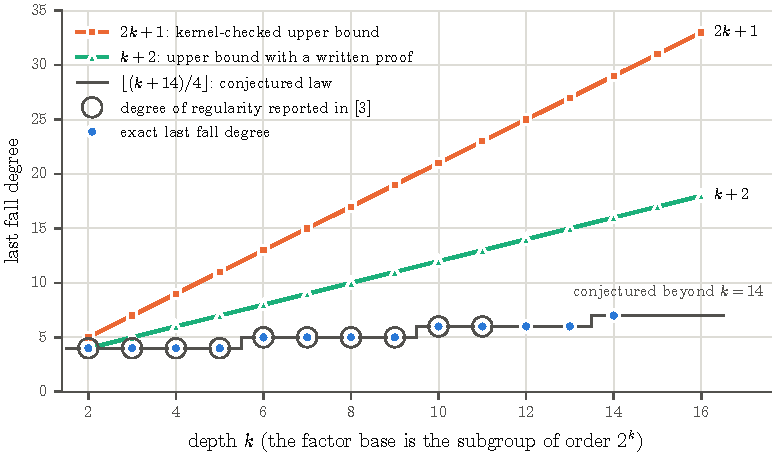
\includegraphics[width=\textwidth]{figures/lfd-depth-profile.pdf}
\caption{The two-summand prime chain profile against the proved bounds.
Dots: exact LFD on the instances computed (Table~\ref{tab:profile}; the
upper bound at $k=14$ is by the degree lift). Rings: the averaged degree of
regularity of Petit, Kosters and Messeng~\cite[Table~4]{pkm}. The step line
is the conjectured law $\lfloor(k+14)/4\rfloor$.}
\label{fig:profile}
\end{figure}

\paragraph{An empirical account of the step at depth six.}
The exact dense closures $V_3$ and $V_4$ of two-summand chain systems were
computed for $k=3,\ldots,10$ on five curves over $p\in\{257,7681,12289\}$
(all five through $k=8$, four at $k=9$, two at $k=10$) with random rational
targets, and
are recorded for every prime system of the sweep. On the five depth-step
curves $\dim V_3=2k+1$; in the sweep this fails only for three systems at
$k=2$ and one at $k=6$, consistent with the kernel-checked
Theorem~\ref{thm:three} above, which excludes $1$ from $V_3$ whenever
$3t^2+a\ne0$. For $k\le5$, $V_4$ is the whole degree-$4$ part of the ideal,
$\dim V_4=|M_{\le4}|-|Z|$, so the certificate holds at degree $4$. For
$k\ge6$ on the depth-step curves, $\dim V_4=4k^2+172k-571$ exactly at
$k=6,\ldots,10$ ($605$, $829$, $1061$, $1301$, $1549$), with
$\dim(V_4\cap M_{\le3})=4k+87$, independent of the prime, the curve and the
number of solutions among these instances. This is not universal: $86$ of
the $333$ prime systems at $k=6,7$ in the sweep deviate, mostly order-two
targets ($607$ and $835$ instead of $605$ and $829$), the $(0,0)$-target
$j=1728$ systems ($730$, $794$, $1343$, $1471$; $1\in V_4$ when $a^{2^k}\ne1$,
kernel-checked), one tangent target with $3t^2+a=0$ ($603$) and one
target of the class $C_2$ of Section~\ref{sec:missing} ($857$). On the generic
instances the quadratic dimension meets the quartic
$|M_{\le4}|=\binom{2k}{\le4}$ between $k=5$ ($389\ge386$, extrapolated) and
$k=6$ ($605<794$): beyond it the degree-$4$ closure cannot contain the
degree-$4$ part of the ideal and $\lfd\ge5$; the matching upper bound $5$ is
the separately measured certificate at degree $5$ for $k\le9$, and it fails
at $k=10$. For $k\ge8$ the identity is bounded above per instance: $V_4(k)$ lies in the free high-level extension of $V_4(7)$, of dimension $829+230(k-7)+2\binom{2k-14}{2}=4k^2+172k-571$ (a written count), by the kernel-checked reduction theorem (Theorem~\ref{thm:reduction}), which turns closedness at depth $8$ into closedness at every depth $k\ge8$. Equality is a computation: it was checked at $k=8,\ldots,12$ on one instance and at $k=8,9$ on two more, and $\dim V_4$ was confirmed through $k=13$ by an independent engine. What
remains open is the genericity of the depth-$7$ base in $(a,b,t)$; with it,
$\lfd\ge5$ would follow for every such system with $|M_{\le4}|-|Z|$ above
the bound.

\begin{figure}[htbp]
\centering
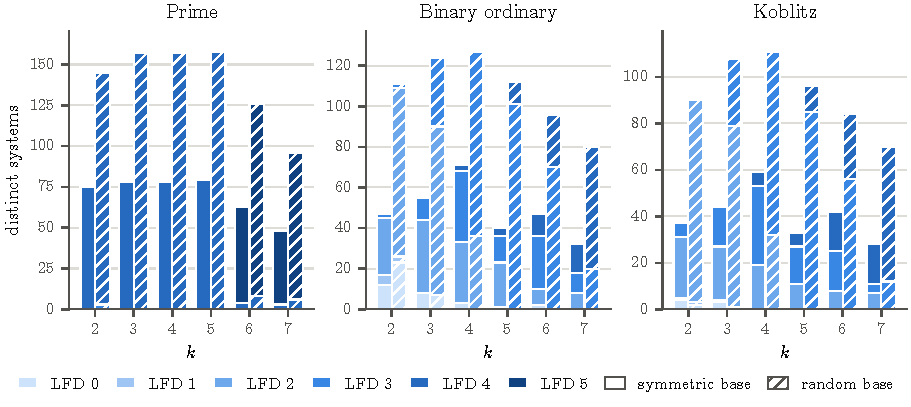
\includegraphics[width=\textwidth]{figures/curve-sweep.pdf}
\caption{Exact LFD in the sweep, by depth or dimension $k$, for each family
(stacked counts of distinct systems). In each pair the left bar is the
symmetric factor base (the subgroup, or a Frobenius-invariant subspace) and
the hatched right bar the random one (a random coset, or a random
subspace).}
\label{fig:sweep}
\end{figure}

\section{What a tight upper bound would need}\label{sec:missing}
The proved bounds are dimension bounds, linear in $k$, while every certified
two-summand value is $3$, $4$ or $5$ for prime chains through $k=9$ (with
$\lfd=6$ on a unit instance at $k=10,\ldots,13$, $\lfd=7$ on it at
$k=14$, and $\lfd\ge6$ on every other instance computed at
$k=10,\ldots,13$) and at most $5$ through $k=10$ for the binary and Koblitz systems computed, which exclude the inverse family with value $\lfloor k/2\rfloor+1$. This section states, as
precisely as the evidence allows, what separates the two.

\paragraph{The mechanism, restated in the group algebra.}
Modulo the chains, the two-summand prime presentation lives in the group
algebra $A=K[G]$, $G=(\mathbb Z/2^k)^2$: a squarefree chain monomial is a
pair of block exponents, its degree is the Hamming weight $\wt(a_1)+\wt(a_2)$,
and multiplication by a chain variable adds $2^j$ to one block exponent.
The normalized generator $g$ has weight at most $2$, the ideal is
$I=gA$, and because the chain ideal is radical with all $4^k$ points
rational, $I$ is the vanishing ideal of the scalar solution set $Z$. The
closure $V_D$ is the smallest subspace of $M_{\le D}$ containing the shifts
of $g$ by exponent patterns of weight at most $D-2$ and closed under
shifting its elements of weight below $D$ by $2^j$; shifts that carry lower
the weight. Carries are not the only source of strict falls: the same
generator closed in the carry-free algebra $K[u]/(u^2)$ still has a fall at
degree $4$. The certificate of
Section~\ref{sec:sweep} says $\lfd\le D$ as soon as
$\dim V_D=|M_{\le D}|-|Z|$ and $M_{<D}$ evaluates onto $Z$.

\paragraph{Generic closure dimensions.}
Write $d_D(k)$ for the dimension of the degree-$D$ closure of a generic
two-summand chain system, the value attained on a Zariski-open set of
coefficient vectors of $g$, if such a value exists. Section~\ref{sec:results}
shows that it cannot be the value for every instance: order-two targets and
the $(0,0)$-target $j=1728$ family have larger $\dim V_4$, and the latter
contains $1$ in $V_4$ at every depth. On the instances we regard as generic
(random curves and random targets of large order), the data are consistent
with $d_3(k)=2k+1$, $d_4(k)=4k^2+172k-571$ for $k=6,\ldots,10$, and
$d_5(k)\ge|M_{\le5}|-|Z|$ for every $k\le9$, where the degree-$5$ closure has
not yet separated from the ideal. For $k=10,\ldots,16$ the computed values are
$d_5=18{,}569$, $25{,}033$, $32{,}057$, $39{,}657$, $47{,}849$, $56{,}649$,
$66{,}073$, and on the
unit instance over $p=65537$ the degree-$6$ closure is $M_{\le6}$ for
$k\le13$ and has dimension $448{,}922<|M_{\le6}|$ at $k=14$, where the
degree-$7$ closure is $M_{\le7}$.

\paragraph{The conjectural formula.}
If the closures of an instance attain the generic values, the local-to-global
certificate gives an upper bound at the first degree where they meet the
ideal, and the dimension count a lower bound below it:
\[
 \lfd(k)=\min\{D:\ d_D(k)=|M_{\le D}|-|Z|\ \text{and}\ M_{<D}\to K^Z\ \text{is onto}\},
\]
up to the strict-fall rule for the exact value. Every tight bound for such
instances is then a statement about the functions $d_D$. Conjecturally, if
$d_D$ is a polynomial of degree below $D$, it cannot keep pace with
$\binom{2k}{\le D}$ and a step beyond $D$ occurs at the first depth $k_0$ at
which $d_D(k_0)<\binom{2k_0}{\le D}-|Z|$. The first such depths computed are
$k_0=2,6,10,14$ for $D=3,4,5,6$, that is $4D-10$
(Figure~\ref{fig:share}), and
$d_5$ is a cubic on the computed range (the recursion below).

\begin{figure}[htbp]
\centering
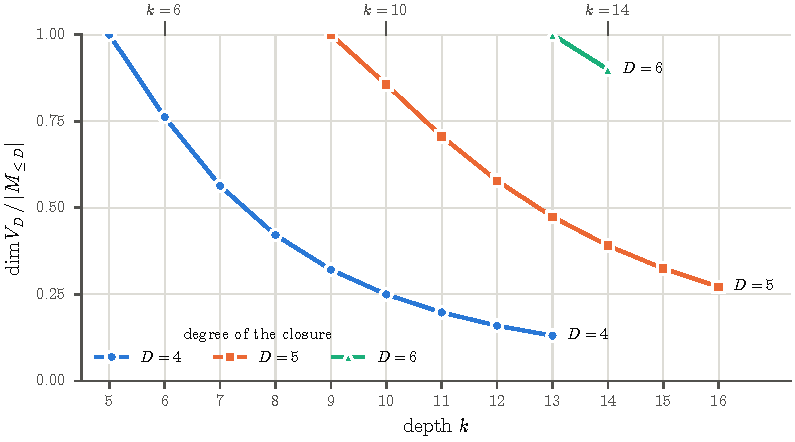
\includegraphics[width=\textwidth]{figures/lfd-closure-share.pdf}
\caption{Share of the degree-$D$ space $M_{\le D}$ reached by the closure
$V_D$ on unit-ideal instances, for $D=4,5,6$. Each curve starts at the last
depth at which the closure is the whole space. The first deficient depths
are $6$, $10$ and $14$, that is $4D-10$. The values for $D=4$ are the
identity $\dim V_4=4k^2+172k-571$; those for $D=5$ and $D=6$ are the
closures of this section (at $k=16$ on the random curve).}
\label{fig:share}
\end{figure}

\paragraph{The depth-ten measurement.}
We computed instances at $k=10$. The first is $p=12289$, $y^2=x^3+x$ (the
$j=1728$ curve), a random rational target (abscissa $9362$, not of order two)
whose two-summand system has no scalar solution, so its ideal is the unit
ideal and $|M_{\le5}|-|Z|=21{,}700$. The exact dense $V_4$ has dimension
$1549=d_4(10)$, matching the quadratic. The degree-$5$ shift closure, with
every low pivot processed once, stops at rank $18{,}569$ after $17$ rounds;
re-reducing all $2k=20$ variable shifts of all $3163$ echelon rows of weight
below $5$ against the final basis adds nothing, so the row space is closed
under every admissible product and is exactly $V_5$. It has codimension
$3131$ in $M_{\le5}$ and does not contain $1$. Since $1$ lies in the ideal,
$\lfd\ge6$ for this system. The conclusion does not depend on the
unit-ideal claim: the system has at most $2\cdot1024$ scalar solutions, so
$\dim(I\cap M_{\le5})\ge21{,}700-2048=19{,}652>18{,}569$ in any case. For
this instance $\dim V_5=18{,}569$; it equals $d_5(10)$ if the instance is
generic. The degree-$5$ closure has separated from the ideal at $k=10$,
whereas it was full on every instance computed at $k=9$; this is consistent
with, not predicted by, the dimension account. An independent rerun from scratch is reported in
Section~\ref{sec:replay}. \DEPTHTENMORE

\paragraph{Three summands.}
For $m=3$ the direct presentation $\{3k\ \text{chains},\ \NF(S_4(x_1,x_2,x_3,t))\}$,
with $S_4=\operatorname{Res}_X(S_3(x_1,x_2,X),S_3(x_3,t,X))$, has exact LFD $7$
at $k=3$ and $4$ on all $234$ seeded cases (five primes, six curves, up to
four targets), and $7=3k+1$ at $k=2$ in $105$ of $116$ cases, so the
kernel-checked bound $mk+1$ is attained there
($1092$ values were recomputed by an independent implementation). The exceptions have $\deg\NF(S_4)=5$, which happens exactly when
the coefficient $-8(5t^3+3at+6b)$ of $x_1^3x_2^3x_3^3$ vanishes.

\begin{theorem}[Carry lower bound; kernel-checked]\label{thm:carry}
Let $G$ be a reduced-ideal-trivial set with $0\notin G$, $g$ a reduced polynomial of degree
$d$, and $h$ a reduced polynomial of degree at most $d$ with
$h-a\,g\in\langle G\rangle$ for some $a$ and $h\ne c\,g$ for every constant
$c$. Then $\lfd(G\cup\{g\})\ge d+1$. For three summands, every field with
$2\ne0$, every depth $k\ge3$ and $5t^3+3at+6b\ne0$, the direct system
$G_{3,k}\cup\{\NF(S_4)\}$ has $\lfd\ge7$.
\end{theorem}
\begin{proof}
By \code{FiniteQuotient.closure\_le\_quotient\_span}, $V_d$ lies in
$(\langle G\rangle\cap M_{\le d})+K g$; if $h$ were there, the reduced
element $h-cg$ would lie in $\langle G\rangle$ and vanish
(\code{CarryLower.not\_hasLFDBound\_of\_carry},
\code{chain\_carry\_lower}). For $m=3$ take $g=\NF(S_4)$, of degree exactly
$6$ because $(3,3,3)$ is its only possible weight-$6$ chain mask, and
$h=\NF(u_{1,0}\,g)$, of degree at most $6$. For $k\ge3$ every exponent of
$S_4$ and $x_1S_4$ is below $2^k$, so the chain normal form is injective on
these supports and $h=cg$ would force $x_1S_4=cS_4$, i.e.\ $S_4=0$. The
expansion of $S_4$ ($125$ coefficients) and its $(3,3,3)$ coefficient are
proved by \code{ring} (\code{M3CarryLower.m3\_lfd\_ge\_seven},
\code{prime\_field\_m3\_lfd\_ge\_seven}).
\end{proof} The
split presentation with a free auxiliary variable has LFD $6$ at $k=4$ and
in $111$ of $117$ cases at $k=3$ ($5$ in the other six).

The value does not move with the depth in the range we can reach. On twelve
further instances (eight primes with $32\mid p-1$, random curves, random and
planted generic targets, the same curve and target at every depth) the
exact LFD is $7$ at every $k=2,\ldots,5$: $V_6$ is spanned by the generator alone,
and $V_7$ is the whole degree-$7$ part of the ideal, $\dim
V_7=|M_{\le7}|-|Z|$ with $M_{<7}$ evaluating onto $Z$ ($|Z|$ between $12$
and $544$ at $k=5$, where $|M_{\le7}|=16{,}384$). So for three summands, at $k\le5$, the
only fall is at $\deg g+1$, where for two summands it is at $\deg g+2$ and
beyond, and at equal depth the three-summand value is $3$ above the
two-summand value at $k=2,\ldots,5$. No degree from $7$ up falls behind the
ideal at $k\le5$, so the free-extension recursion of the two-summand
closures had nothing to act on there.

At $k=6$ the degree-$7$ closure, computed on one instance, does fall behind
the ideal. The instance is $p=7681$, $y^2=x^3+1876x+2678$, target abscissa
$6223$, with $|Z|=48$ scalar solutions and $|M_{\le7}|=63{,}004$ columns in
$18$ chain variables. Here $V_6=\operatorname{span}(g)$ as at smaller depths,
but $V_7$ is closed, by a deterministic full sweep, with
$\dim V_7=19{,}958$, low profile $(0,0,0,0,0,3,2375)$ and $1\notin V_7$,
against $\dim(I\cap M_{\le7})=62{,}956$. So an element of the ideal of degree
at most $7$ lies outside $V_7$, and
\[
 \lfd\ge8\quad\text{at }k=6
\]
for this instance (an exact computation, on one instance and with one
engine).
This is the first depth at which a three-summand value above $7$ is
established on any instance, and it is the depth at which the two-summand
degree-$4$ closure first falls behind. The exact value at $k=6$ would need the
degree-$8$ closure ($|M_{\le8}|=106{,}762$ columns), which was not computed,
and the only upper bound there is the kernel-checked $3k+1=19$. There is no
computation at $k\ge7$, no replication of the $k=6$ run on a second
instance or engine, and no prediction for the depths beyond $6$.

\paragraph{More summands.}
The two bounds used for three summands apply to every $m$.
Corollary~\ref{cor:allm} gives $\lfd\le mk+1$. The first statement of
Theorem~\ref{thm:carry}, applied to $g=\NF(S_{m+1})$ and $h=\NF(x_1g)$, gives
$\lfd\ge\deg g+1$ whenever $\deg h\le\deg g$ and $h$ is not a constant
multiple of $g$. By Lemma~\ref{lem:degree}, $\deg g\le m\min(k,m-1)$, so the
two bounds can meet only for $k\le m-1$, and they do meet when $g$ has the
full degree $mk$, that is, when the product of all $mk$ chain variables
occurs in $g$.

We computed $g$ exactly for $m=3,\ldots,8$, that is for the summation
polynomials $S_4$ to $S_9$, without expanding $S_{m+1}$. Modulo the chains a
polynomial is a function on $H^m$, so $g$ is the inverse discrete Fourier
transform of the values of $S_{m+1}$ on $H^m$, and these values follow from
Semaev's resultant recursion carried out with numbers. As checks, the values
vanish at $t=x(P_1+\cdots+P_m)$ for random rational points and every
$m\le8$, and for $m=3$ the computation agrees with the generator degree, the
number of solutions and the exact LFD of all $344$ three-summand systems
above with $k\le3$. The instances are over the primes $97$, $193$, $257$,
$7681$, $12289$ and $65537$, on $y^2=x^3+x$, $y^2=x^3+1$ and two random
curves per prime, with two random rational targets per curve.

\begin{table}[htbp]
\centering\small
\begin{tabular}{@{}llccc@{}}
\toprule
$m$ & polynomial & $k=2$ & $k=3$ & $k=4$\\
\midrule
$3$ & $S_4$ & $7$ \ ($48$ of $48$) & & \\
$4$ & $S_5$ & $9$ \ ($48$ of $48$) & $13$ \ ($47$ of $48$) & \\
$5$ & $S_6$ & $11$ \ ($48$ of $48$) & $16$ \ ($48$ of $48$) & $21$ \ ($8$ of $8$)\\
$6$ & $S_7$ & $13$ \ ($48$ of $48$) & $19$ \ ($8$ of $8$) & $25$ \ ($2$ of $2$)\\
$7$ & $S_8$ & $15$ \ ($47$ of $48$) & $22$ \ ($8$ of $8$) & ---\\
$8$ & $S_9$ & $17$ \ ($47$ of $48$) & $25$ \ ($2$ of $2$) & ---\\
\bottomrule
\end{tabular}
\caption{Exact LFD $mk+1$ of the direct $m$-summand prime chain system at
depth $k\le m-1$, with the number of instances on which it is established.
Dashes: not computed (more than $2^{24}$ grid points).}
\label{tab:msum}
\end{table}

\begin{figure}[htbp]
\centering
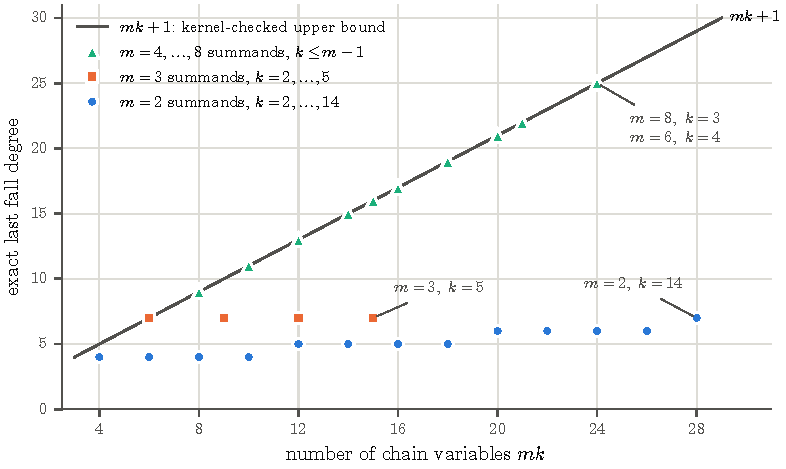
\includegraphics[width=\textwidth]{figures/lfd-variables.pdf}
\caption{Exact LFD against the number $mk$ of chain variables. With
$m\ge4$ summands at depth $k\le m-1$ (triangles, Table~\ref{tab:msum}) and
with three summands at $k=2$, the value lies on the bound $mk+1$. With three
summands at $k=3,4,5$ (squares) and with two summands (dots,
Table~\ref{tab:profile}) it stays far below.}
\label{fig:variables}
\end{figure}

On $409$ of the $412$ instances with $2\le k\le m-1$ the generator has
degree $mk$ and the two hypotheses on $h$ hold, so $\lfd=mk+1$ exactly
(Table~\ref{tab:msum}, Figure~\ref{fig:variables}). The dimension bound is therefore attained by
summation systems themselves for every $m$ from $3$ to $8$, with values up
to $25$, and not only by the abstract Boolean family of Table~\ref{tab:bounds}. The attainment is of the simplest kind: at budget $\deg g$ the generator cannot be multiplied, so the lower bound is one more than the input degree, and with $\deg g=mk$ it meets the upper bound $\max(mk+1,\delta)$. These systems have one fall, directly above the input degree; the agreement says nothing about how the closures grow, and it is not comparable with the two-summand profile, whose falls lie above $\deg g+1$. The three exceptions are unit ideals on
$y^2=x^3+x$ with $\deg g=mk-1$; the argument decides nothing for them. For
$k\ge m$ the generator has degree $m(m-1)$ on every instance computed, which
gives $\lfd\ge m(m-1)+1$: the bound $7$ for three summands at $k=3,4$
($96$ instances), in agreement with the exact values above, and
$\lfd\ge13$ for four summands at $k=4,5$ ($56$ instances), where the upper
bounds are $17$ and $21$. For $m\ge4$ the lower bounds use the kernel-checked
statement with hypotheses established by this exact computation and not by
the kernel. The largest cases rest on few instances (sixteen with $2^{20}$ or $2^{21}$ grid points, four with $2^{24}$), depths with more than $2^{24}$
grid points were not computed, and no exact value is known for $k\ge m$
when $m\ge4$.

\paragraph{The chain bridge and the depth reduction.}
Two kernel-checked statements turn the group-algebra computations of this
section into statements about the ordinary closure. Write $\NF$ for the
graded remainder modulo the chains and $V^{q}_D(F)$ for the closure in the
reduced space under the rule $w\mapsto\NF(x\,w)$ for $\deg w<D$.

\begin{theorem}[Chain bridge; kernel-checked]\label{thm:bridge}
For every field with $2\ne0$, all $m,k$, every input set
$F=G_{m,k}\cup R$ and every $D\ge2$: $p\in V_D(F)$ if and only if
$\deg p\le D$ and $\NF(p)\in V^{q}_D(F)$ (\code{ChainClosureBridge.chain\_mem\_closure\_iff}).
\end{theorem}
The direct-sum form $V_D(F)=(\langle G_{m,k}\rangle\cap M_{\le D})\oplus V^{q}_D(F)$ follows at once; it is written, not a separate Lean declaration.

This proves the premise used throughout the computations, that working
modulo the chains gives the ordinary closure for $D\ge2$, which had been
checked only numerically. The second statement is the reduction of all
depths to one finite base. For a base depth $k_0$, a degree $D$ and a subspace $S$ of the depth-$k_0$ chain algebra in degree at most $D$, let $W_k(S)=\bigoplus_q\tau_q(S\cap M_{\le D-\wt q})$, the sum over high exponent patterns $q$ on levels $k_0,\ldots,k-1$ of the translates of $S$. Below, $k_0=7$ and $D=4$ unless stated otherwise.

\begin{theorem}[Depth reduction; kernel-checked]\label{thm:reduction}
Let $K$ be a field with $2\ne0$. For every subspace $S$ and all $k_0,D,m$: if $W_{k_0+1}(S)$ is closed under
the admissible variable products at depth $k_0+1$, then $W_k(S)$ is closed
at every depth $k\ge k_0+1$, and $1\in W_k(S)$ if and only if $1\in S$
(\code{DepthReduction.W\_closed}, \code{single\_zero\_mem\_W\_iff}). If moreover $S$ contains the generator, then the normal forms of $V_D(k)$ lie in $W_k(S)$ for every $k\ge k_0+1$ (\code{ShiftWitness.normalForm\_mem\_map\_W}). Consequently, for two-summand prime chain systems: if some $S$ at depth $7$
contains the generator, excludes $1$, and has $W_8(S)$ closed, then
$1\notin V_4$ at every depth $k\ge8$, and a unit ideal has $\lfd\ge5$ at
every depth $k\ge8$ (\code{ChainModelMap.n5\_lfd\_ge\_five},
\code{prime\_field\_n5\_lfd\_ge\_five}).
\end{theorem}

The hypotheses are three finite facts about one depth-$7$ space. For two
concrete instances the kernel checks them without \code{native\_decide}:
$p=40961$ with $(a,b,t)=(21223,9887,4748)$, where $S=V_4(7)$ has dimension
$829$ in $1471$ columns, and a small analogue $p=11$, $(a,b,t)=(2,5,7)$, with
the same dimension profile. The certificate packs each echelon row into one
large integer, so that a membership test is a few big-integer
multiply-and-adds followed by a check of each free slot modulo $p$. The
closedness of $W_8(S)$ reduces, through the component formulas of the
reduction, to $3220$ such memberships at depth $7$, about $2\cdot10^7$
kernel operations, which run in about $14$ minutes per instance in $42$ \code{decide +kernel} chunks. The result is unconditional for these
instances: $1\notin V_4(k)$ at every depth $k\ge8$
(\code{N5CertInstanceP40961.not\_one\_in\_closure},
\code{N5CertInstanceP11.not\_one\_in\_closure}).

The lower bound itself needs no assumption on the ideal. By definition,
$\lfd>D$ as soon as one ideal element of degree at most $D$ lies outside
$V_D$, and an element of the low box outside $S$ stays outside $W_k(S)$ at
every depth. No single shifted generator $x_1^{e_1}x_2^{e_2}g$ of weight at
most $4$ is such an element (all $131$ candidates with $e_i\le125$ lie in
$V_4(7)$), but a combination $h\,g$ with $\deg h=(46,46)$ is: it has weight
at most $4$, $161$ monomials, and a nonzero echelon residual. The
kernel checks the product in chunks and the residual, which gives, with no
hypothesis left,
\[
 \lfd\ge5\quad\text{at every depth }k\ge8
\]
for $p=40961$, $(a,b,t)=(21223,9887,4748)$ and for $p=11$, $(2,5,7)$, as statements about these polynomial systems at every depth. They are subgroup systems only where $2^k\mid p-1$: for $p=40961$ that is $k\le13$, beyond which the statement concerns the same system over an extension field; $p=11$ has no subgroup of order $2^k$ for $k\ge2$, and $t=7$ is not the abscissa of a rational point of $y^2=x^3+2x+5$, so that instance is a test polynomial system rather than a summation system over $\F_{11}$;
the Lean statements are \code{lfd\_ge\_five} in the modules
\code{N5CertWitnessInstanceP40961} and \code{N5CertWitnessInstanceP11}. The
same statement for any
degree $D$ and base depth $k_0$, conditional on one base certificate per $D$ and with $k_0\ge2$, is \code{GrowthSchema.growth\_schema}; only $D=4$, $k_0=7$ is
certified.

\begin{theorem}[An exact value above four; kernel-checked]\label{thm:exactsix}
For $p=1153$, the curve $y^2=x^3+139x+1094$ and the target abscissa
$t=185$, the two-summand chain system at depth $k=6$ has last fall degree
exactly $5$ (\code{ExactK6InstanceP1153.exact\_lfd\_five}).
\end{theorem}

This is the first value of the measured profile above $4$ that the kernel
checks from both sides; the ideal is the unit ideal, which the upper
certificate proves and does not assume. The upper half is a derivation of
$1$ inside $V_5$ of $83$ rows and $39{,}126$ terms, each row a combination
of variable shifts of earlier rows within the degree budget; a vector is one
big integer with $128\times128$ slots, so a shift is a multiplication by a
power of two, and the wrap $x^{64}=1$ is folded once per row. The lower half
is the containing space $S=V_4(6)$, of dimension $605$, with all $1332$
shifts of its $111$ low rows tested for membership as in the depth-$7$
certificate. The kernel work is about twelve minutes in $125$
\code{decide +kernel} theorems. The instance was the first unit ideal of a
seeded search (small primes with $64\mid p-1$ almost never give unit ideals
at depth $6$, since about $4096/p$ solutions are expected); its closure
dimensions $(0,0,2,111,605)$ and $\dim V_5=1586=|M_{\le5}|$ are the generic
depth-$6$ values. It is one instance: the generic value $5$ at depth $6$
remains a certified computation.

\begin{theorem}[Depth restriction; kernel-checked]\label{thm:restrict}
For every field, all $a,b,t$, every $k\ge2$ and $D\ge2$: the substitution
$u_{i,k}\mapsto1$ maps the degree-$D$ closure at depth $k+1$ into the
degree-$D$ closure at depth $k$. Hence $1\in V_D(k+1)$ implies
$1\in V_D(k)$, and an exclusion $1\notin V_D(k_0)$ holds at every depth $k\ge k_0$ (\code{DepthRestrictionM2.restrict\_closure}, \code{not\_one\_of\_le}, \code{lfd\_gt\_of\_le}). As a short written corollary, not a Lean declaration, the last fall degree is nondecreasing in the depth over any range of depths on which the ideal is the unit ideal.
\end{theorem}

The substitution sends the chain equations of depth $k+1$ to those of depth
$k$ or to zero and fixes the generator, so it maps derivations to
derivations without raising degrees. Applied to
Theorem~\ref{thm:exactsix} it gives, in the kernel, $1\notin V_4(k)$ at every
depth $k\ge6$ for that instance
(\code{ExactK6Deeper.not\_one\_in\_closure\_four\_of\_ge}). With the certified exclusion
$1\notin V_5(10)$ on the unit instance, Theorem~\ref{thm:restrict} gives
$1\notin V_5(k)$ for every $k\ge10$ for the same coefficients $(a,b,t)$; the
base fact is a certified computation, not a kernel certificate, and beyond
$k=12$ the system over $\F_{12289}$ is no longer a subgroup system
($2^{13}\nmid p-1$), so there the statement concerns the same polynomial
system over an extension field. Likewise the exclusion $1\notin V_6(14)$ on the unit instance over $p=65537$
gives $1\notin V_6(k)$ for every $k\ge14$ for the same coefficients (subgroup
systems for $k\le16$). For unit ideals the theorem also reduces the
growth law $\lfd(k)=\lfloor(k+14)/4\rfloor$ suggested by the profile to two
finite statements per degree, $1\in V_D(4D-11)$ and $1\notin V_D(4D-10)$;
they hold for $D=4,5,6$ on the computed unit instances ($1\in V_6(13)$ and
$1\notin V_6(14)$ on the unit instances over $p=65537$ and $p=163841$) and
are open from
$D=7$ on, where the first test, $1\in V_7(17)$ against $1\notin V_7(18)$,
is far beyond the present engines; the lift gives $1\in V_7(14)$ on both unit
instances, which $1\in V_7(17)$ would imply.

\paragraph{What is missing, in order of difficulty.}
\begin{enumerate}
\item \emph{A genericity theorem.} A proof that for $k$ above a threshold
 the row reduction of the degree-$D$ closure never pivots on a quantity
 that vanishes for an actual curve and target outside an explicit
 exceptional locus, so that $\dim V_D=d_D(k)$ there. The locus must contain
 the order-two targets and the $(0,0)$-target $j=1728$ family, where
 $\dim V_4$ is larger (Section~\ref{sec:results}). A natural route is to run
 the closure over the polynomial ring in the coefficients of $g$ and identify
 the pivots as polynomials in $a$, $b$, $t$; the top coefficients of $S_3$
 are $1$, $-2(t^2+a)$ and $-2t$, so already the degree-$3$ analysis needs
 $3t^2+a\ne0$ (Theorem~\ref{thm:three}). At $k=6$ and $p=193$ the exceptional set among the targets computed is known (it was re-verified on a stratified
sample of $96$ targets including every deviating one): over $1276$ targets on $13$ curves the exact
 LFD is $5$ except for $12$ targets with value $4$, which are exactly those
 with $t=0$ and $ab=0$ ($3$) or with normalized point $(a/t^2,b/t^3)$ in a
 set $C_2$ of $190$ points of the plane ($9$); $C_2$ lies on no curve of degree at most $18$, which carries little information, since $190$ points in general position lie on no such curve; a cubic $C_1$ and the tangent line $3t^2+a=0$ change the
 closure dimensions but not the LFD.
 On one $C_2$-class target at $k=7$ ($p=257$) the exact LFD is $5$, so the
 exceptional set depends on the depth at least there, and if $C_2$ is not the
 reduction of a curve the theorem must be stated prime by prime.
 An analysis of this item (with written proofs, not kernel-checked) gives three conclusions. First, the computed closure dimensions lie on both sides of $605$ (order-two targets $607$, the tangent line $603$). Rigorously, only the drop below the computed value on the line $b=t=0$ is established; if $605$ is the generic value, as conjectured, the dimension is semicontinuous in neither direction, and the generic facts cannot be inferred from computed points; what is needed is the generic depth-$7$
 basis over $\F_p(a/t^2,b/t^3)$, whose common denominator has degree at least $480$ along a random line of the plane (an exact lower bound at $k=6$ and $7$, whose records are not in the repository), a certificate of an estimated $10^{10}$ coefficients that is out of reach of the kernel. Second,
 full invariance of the closure dimension under $(a,b,t)\mapsto(\mu^2a,\mu^3b,\mu
 t)$ fails for $\mu\notin H$ ($730$ against $794$ on the $t=b=0$ line at
 $p=193$), but the depth-$8$ certificate is invariant: scaling by $\mu$ is
 the same system with the coset $\mu^{-1}H$ as factor base, and the free
 extension $W_k(S)$ remains closed in every twisted algebra. Hence one point
 that passes the depth-$7$/$8$ certificate gives $\lfd\ge5$ at every depth $k\ge8$, as polynomial systems (subgroup systems only while $2^k\mid p-1$, so $k\le6$ at $p=193$), on its whole orbit of $p-1$ scalings (unit ideals; proper ideals
 when $|Z|$ is below the dimension gap). Third, the strongest exact
 description of the exceptional set within reach is per prime: the certificate at all $37{,}249$ points of the plane at $p=193$ is estimated at about $52$ CPU-hours.
\item \emph{The polynomials $d_D(k)$.} For $D=3$ the kernel-checked
 Theorem~\ref{thm:three} proves the consequence that matters, $1\notin V_3$
 at every depth when $3t^2+a\ne0$, by showing that no combination of $g$ and
 its multiples by a variable falls below degree $3$. For $D=4$ the identity $4k^2+172k-571$ is an upper bound per instance for $k\ge8$, by the free high-level extension of $V_4(7)$, and an equality on the computed range (Section~\ref{sec:results}); a
 parametric description of $V_4(7)$, of dimension $829$ with a fall of
 dimension $2k+86$ above $V_3$ in the low part, is still missing. For $D=5$ the closure is full through $k=9$ and
 $\dim V_5=18{,}569$, $25{,}033$, $32{,}057$, $39{,}657$, $47{,}849$,
 $56{,}649$, $66{,}073$ at
 $k=10,\ldots,16$ satisfy the exact recursion of
 Section~\ref{sec:missing}, so $d_5$ is a cubic on the computed range; whether
 the recursion holds beyond $k=16$ is untested. For $D=6$ the closure is
 full through $k=13$ and has dimension $448{,}922$ at $k=14$ on four instances; the deficient codimensions $10$, $189$, $3131$, $50{,}256$ at the first
 deficient depths $4D-10$ have no formula.
\item \emph{A lower bound outside the exceptional locus.} An upper bound
 $\dim V_4\le f(k)$ with $f$ quadratic cannot hold for every instance
 (\code{PrimeM2Sharp.one\_at\_four} puts $1\in V_4$ at every depth on the
 $(0,0)$-target family). Proved for all instances outside an explicit
 exceptional locus, it would give $\lfd\ge5$ for every such system with
 $|M_{\le4}|-|Z|>f(k)$, by the exclusion principle of
 \code{QuotientLowerBound}. Per instance, Theorem~\ref{thm:reduction}
 reduces it to three finite facts at depth $7$ and $8$, and the kernel
 checks them for concrete instances and proves $\lfd\ge5$ there at every
 depth $k\ge8$ without further hypotheses (above). What is missing is their
 genericity in $(a,b,t)$ (item~1), and a base certificate for each degree
 $D\ge5$ in the growth schema.
\item \emph{A tight upper bound.} $\lfd\le5$ for all $k<k_0$ needs
 $d_5(k)\ge\binom{2k}{\le5}-|Z|$, i.e.\ a spanning argument: every
 weight-$\le5$ polynomial vanishing on $Z$ must be exhibited as a degree-$5$
 derivation. Because the shifts of $g$ alone span only
 $O(k^3)$ dimensions, the derivation must pass through the fall space
 $V_5\cap M_{<5}$ and its shifts; a structural description of that fall
 space (which carries, from which exponent patterns) is the missing object.
 The dense final certificates show it exists for $k\le9$ but do not
 describe it, and the depth-ten measurement shows that no such argument can
 extend to every $k$: the bound $\lfd\le5$ fails at $k=10$. The proved
 upper bounds have slope $1$ in $k$ (Theorem~\ref{thm:selector}) and the
 measured profile has slope about $\tfrac14$; closing that gap needs, for
 each degree $D$, the statement $1\in V_D(4D-11)$ of
 Theorem~\ref{thm:restrict} and its analogue for proper ideals, and we found
 no inductive mechanism relating $V_D(k)$ to $V_{D+1}(k+4)$. The statement
 $1\in V_6(13)$ and the exclusion $1\notin V_6(14)$ are now measured on two
 unit instances. The exact value $7$ at $k=14$ comes from the degree lift, on
 both of them and on a random curve; a direct closure in $M_{\le7}$ at that
 depth, which would certify it, is out of reach.
\item \emph{Binary and Koblitz.} The written $\min(k,\ell)+2$ bound is
 tight in order but not in constant; the measured two-summand values on the grids are at most $5$ through $k=10$, and the inverse family (a Koblitz curve) has $6$ at $k=10$. On the first grid the $28$ systems with value $5$, all at $k=10$,
 were exactly those with more than $470$ solutions. A follow-up shows that this is not a law. Every
 equation is affine bilinear in the two coordinate blocks and the curve
 coefficient $a$ does not occur; for a target with $x_R\ne0$ the trace form
 $\operatorname{Tr}(\cdot/x_R^2)$ gives one linear equation, which is why a
 trace-zero coordinate space doubles or empties the solution set. Two
 candidate laws were fixed before $80$ new cases ($75$ distinct systems) were run: the value as a
 function of the expected log-count $e$ of solutions alone, and as a
 function of $k+e$. Both are refuted ($11$ hits against $36$ misses, and
 $36$ against $11$, on the $47$ systems chosen to separate them): a
 trace-zero hyperplane at $k=9$ with about $490$ solutions has value $5$ in
 $11$ of $11$ systems, and unit ideals reach $4$ at $k=7$. There is no bound
 in the solution count alone, and the subfield $\F_{2^8}\subset\F_{2^{16}}$
 with $255$ solutions has value $5$ at $k=8$, the inverse-family value
 $k/2+1$. A two-term rule (a floor that grows with $k$ and a term that grows
 with the solution count) fits the old and new data but was chosen after the
 check, so it is a conjecture. The pre-certificate closure dimensions depend only on $(n,k)$, the target class and two effective-dimension fields of the record in $1678$ of $1775$ systems. A tight
 bound must therefore depend on the coordinate space and on $k$, not only on
 the solution count or the dimension. The kernel
 specialization of the selector theorem is the open formal item of the
 companion manuscript.
\end{enumerate}

\section{Independent checks}\label{sec:replay}
\REPLAYTEXT

\section{Related work}\label{sec:related}
The last fall degree was introduced by Huang, Kosters and Yeo~\cite{hky15}; the closure framework used here is that of Huang, Kosters, Yang and Yeo~\cite{hkyy}, who also show that solving cost depends on the LFD together
with the number of solutions~\cite[Prop.~2.8]{hkyy}; Caminata and
Gorla~\cite{cg} relate LFD to solving degree and the degree of regularity,
and their Theorem~2.9 and Example~4.3 give LFD $0$ for a Gr\"obner basis,
the case $k=1$ of the chain system. LFD bounds for Weil-descent systems are
due to Huang, Kosters and Yeo~\cite{hky15}, Huang~\cite{huang21} and
Gorla, Mueller and Petit~\cite{gmp21}; Steiner~\cite{steiner24} uses the same
coprime-leading-term structure to bound solving degrees of iterated systems.

The prime two-power subgroup presentation is due to Petit, Kosters and
Messeng~\cite[\S3.3]{pkm}. Their Table~4 reports Magma's corrected degree
of regularity for the same two-summand subgroup-chain presentation, averaged
over $100$ random instances per depth (the smallest prime $p$ with
$2^{n_1}\mid p-1$ and $p\ge2^{2n_1}$, a random curve and point, about one
solution per instance): $4.00$ for $n_1\le5$, $5.00$ for $n_1=6,\ldots,9$
and $6.00$ for $n_1=10,11$, without an explanation; their Table~5
(isogeny-kernel factor bases) shows $5$ up to kernels of order $2^9$ and $6$
at $2^{10}$ and $2^{11}$. The breakpoints coincide with the exact LFD values certified
here, which suggests that LFD, and not a solver artefact, is behind their
table; our contribution on this point is the exact certified value (rather
than a solver step degree), the exact value $6$ on one unit instance at
$k=10,\ldots,13$ (their $n_1=10,11$ are the first two), the bound
$\lfd\ge7$ and the lifted value $7$ at $k=14$ on it, and the dimension account of
Section~\ref{sec:results}. Kousidis and
Wiemers~\cite{kw19} study first fall degrees of summation polynomials.

Linear-subspace factor bases go back to Diem~\cite{diem11} and Petit and Quisquater~\cite{pq12}; the binary descent with linear coordinate spaces used here is from Faug\`ere, Perret, Petit and Renault~\cite{fppr} after Semaev~\cite{semaev}; symmetrized
summation polynomials and small-order torsion are in Faug\`ere, Huot, Joux,
Renault and Vitse~\cite{fhjrv}, and automorphism symmetries in Faug\`ere,
Gaudry, Huot and Renault~\cite{fghr14}. Kosters and Yeo~\cite{ky} prove that
the first fall degree of ordinary binary $S_3$ systems is $2$, show that
evaluating summation polynomials is NP-complete, and observe that the degree
of regularity grows with $n$ and depends on the choice of coordinate space
(their Section~5). Galbraith, Granger, Merz and Petit~\cite{ggmp21} show that
Frobenius-invariant factor bases reduce the number of systems and the
linear-algebra cost for subfield and Koblitz curves; our finding that the
LFD differences of such bases follow the solution count (Section~\ref{sec:results}) concerns the degree of a
single system and leaves their savings untouched. Galbraith and
Gebregiyorgis~\cite{gg} report Gr\"obner-basis experiments for binary curves.

Gr\"obner bases have been formalized in Coq~\cite{thery01}, Isabelle/HOL
\cite{maletzky-immler18} and Lean~\cite{guo26}; we are not aware of a
formalization of last fall degree, first fall degree or solving degree. The
dimension bound $mk+1$ is the generic finite-quotient bound and is not new
as a bound; what is new is the kernel-checked statement for every input list
containing the chains, and its two-summand corollary at every depth.

The Lean development (Lean~4.19.0 with Mathlib) has \LEANDECLS{} audited
declarations. They depend only on the foundational axioms \code{propext},
\code{Classical.choice} and \code{Quot.sound}, and use no further axioms, no
\code{sorry} and no \code{native\_decide}. The certificates of the sweep are
exact arithmetic and can be replayed. The Lean development contains no elliptic curve: $S_3$ and $S_4$ enter as explicit polynomials, which are not proved there to be summation polynomials, and the binary and Koblitz bounds are one generic Boolean theorem, the second being the first with $b=1$. The local-to-global step for prime chains is the same rank argument as the Boolean one; it is applied by hand
and is not an instance of the kernel theorem.

\section{Conclusion}
For the three presentations of elliptic-curve summation systems studied
here, the last fall degree is at most the finite-quotient bound $mk+1$; for
prime chains this is kernel-checked at every depth and for every number of
summands. A written proof lowers the two-summand prime bound to $k+2$ on
nonsingular curves. From below, $\lfd\ge4$ holds at every depth for
two-summand prime chain systems with unit ideal and $3t^2+a\ne0$, and
$\lfd\ge7$ for three summands at every depth $k\ge3$ when
$5t^3+3at+6b\ne0$; both are kernel-checked.

For two summands the exact values are much smaller than the upper bounds.
Over prime fields they are $4$, $5$, $6$ and $7$ on the depth ranges
$2$--$5$, $6$--$9$, $10$--$13$ and $14$, with the exceptions of
Section~\ref{sec:results}; they reproduce the degree-of-regularity
breakpoints of Petit, Kosters and Messeng and extend them by three depths.
The value at $k=14$ depends on a degree lift without an independent
certificate, and every depth beyond $14$ is open. The law
$\lfd(k)=\lfloor(k+14)/4\rfloor$ fits all of these values and remains a
conjecture. With three summands the value is $7$ through $k=5$ and at least
$8$ on one instance at $k=6$. With three to eight summands and depth
$k\le m-1$ the bound $mk+1$ is attained on the instances computed. For binary and Koblitz curves the value is at most $5$ through dimension $10$ on the grids computed, while the structured inverse family grows as $\lfloor k/2\rfloor+1$, and the differences between random and
Frobenius-invariant factor bases follow the number of solutions on our grid,
which is an association and not a causal statement.

For two summands a tight upper bound is not proved: the proved bounds grow with slope $1$ in
$k$ and the measured values with slope about $\tfrac14$.
Section~\ref{sec:missing} lists what closing this gap would need.

\section{Code and data}\label{sec:artifacts}
The Lean development, the closure engines, the independent checker, the
written proofs and the records behind the numbers in this paper are in the companion repository, except where the text says that records were not kept (the selector-bound test, the genericity denominator, and the $k=14$ degree-$6$ bases)
\begin{center}
\url{https://github.com/isogeny-labs/lfd-summation-systems}
\end{center}
Paths are relative to its root.

\begin{center}\small
\begin{tabular}{@{}>{\raggedright\arraybackslash}p{6.6cm}>{\raggedright\arraybackslash}p{8.4cm}@{}}
\toprule
Material & Location\\
\midrule
Lean development, its audit and certificate data & \code{formal/}, \code{experiments/\allowbreak{}ic-lean/}, \code{ic-bounds-cert/}, \code{ic-bounds-exact-k6/}\\
Sweep (Sections~\ref{sec:sweep} and~\ref{sec:results}) & \code{experiments/\allowbreak{}ic-curve-sweep/}\\
Depths $8$, $9$ and $10$ & \code{experiments/\allowbreak{}ic-chain-depth8/}, \code{-depth9/}, \code{-depth10/}\\
Independent engine, depths $10$ to $13$; $\dim V_4$ & \code{experiments/\allowbreak{}ic-bounds-d5/}, \code{ic-bounds-exact10/}, \code{ic-bounds-fall/}\\
GPU engine, degree lift and checker, depths $10$ to $16$ & \code{experiments/\allowbreak{}ic-bounds-k14/}\\
Free extension and predictions & \code{experiments/\allowbreak{}ic-bounds-freeext/}\\
Three summands & \code{experiments/\allowbreak{}ic-bounds-m3/}, \code{ic-bounds-m3-depth/}\\
Three to eight summands & \code{experiments/\allowbreak{}ic-bounds-msum/}\\
Exceptional locus at $k=6$ & \code{experiments/\allowbreak{}ic-bounds-locus/}\\
Depth-step table ($\dim V_3$, $\dim V_4$, $k=3,\ldots,10$) & \code{experiments/\allowbreak{}ic-depth-step/}\\
Binary and Koblitz follow-up & \code{experiments/\allowbreak{}ic-bounds-binary/}, \code{ic-bounds-binary-law/}\\
Independent ordinary-ring validator & \code{experiments/\allowbreak{}ic-curve-validation/}\\
Written proofs and their reviews & \code{docs/\allowbreak{}proofs/}, \code{docs/\allowbreak{}reviews-*.md}\\
\bottomrule
\end{tabular}
\end{center}

The main computations are reproduced by the following commands.
\begin{verbatim}
python scripts/verify_lean_fall_degrees.py --lake /path/to/lake
python scripts/run_ic_curve_sweep.py --check-only
python scripts/run_ic_chain_depth8.py --check-only
python scripts/run_ic_chain_depth8.py --check-only --depths 9 --primes 7681 \
  --out experiments/ic-chain-depth9 --workers 1 --product-cap 12000 \
  --shift-max-cells 450000000
python scripts/run_ic_chain_depth10_probe.py --tag rerun
python scripts/run_ic_chain_depth10_probe.py --prime 13313 --seed 11 \
  --want-solutions --tag proper-13313-replay
python scripts/run_ic_chain_depth10_probe.py --prime 15361 --a 4021 \
  --b 9917 --seed 12 --tag random-15361-replay
python scripts/run_ic_chain_depth10_degree6.py --combos 3000
python scripts/run_ic_depth_step.py
python scripts/analyze_ic_base_classes.py
python scripts/ic_bounds_msum.py run --max-log2-points 24
python scripts/plot_ic_lfd_figures.py
python scripts/build_ic_curve_paper.py
\end{verbatim}
The first command builds the Lean project and prints the axiom dependencies
of every audited declaration. The next three regenerate every case of the
sweep and of the depth-$8$ and depth-$9$ systems and replay every exact
closure. The next three rerun the depth-ten closures (about two hours each)
and the one after that the degree-six closure (about five hours, up to ten
gigabytes). The last five regenerate the depth-step table, the base-class
analysis, the more-summand records, the figures and this document. The runs at depths eleven to
fourteen over $p=65537$ need a GPU (the $k=14$, $D=6$ closure used a card
with $141$ GB and moved part of the basis to host memory); their commands,
and those of the degree lift, are in the \code{README.md} and \code{LIFT.md}
of \code{experiments/\allowbreak{}ic-bounds-k14/}. The three-summand, exceptional-locus
and binary runs are described in the \code{README.md} of their directories.

\begin{thebibliography}{99}
\bibitem{hkyy} M.-D. A. Huang, M. Kosters, Y. Yang and S. L. Yeo.
\emph{On the last fall degree of zero-dimensional Weil descent systems}.
Journal of Symbolic Computation 87 (2018), 207--226.
\href{https://doi.org/10.1016/j.jsc.2017.08.002}{doi:10.1016/j.jsc.2017.08.002}.
\bibitem{cg} A. Caminata and E. Gorla.
\emph{Solving degree, last fall degree, and related invariants}.
Journal of Symbolic Computation 114 (2023), 322--335.
\href{https://arxiv.org/abs/2112.05579}{arXiv:2112.05579}.
\bibitem{pkm} C. Petit, M. Kosters and A. Messeng.
\emph{Algebraic approaches for the elliptic curve discrete logarithm problem over prime fields}.
PKC 2016, LNCS 9615, 3--18.
\href{https://doi.org/10.1007/978-3-662-49387-8_1}{doi:10.1007/978-3-662-49387-8\_1}.
\bibitem{fppr} J.-C. Faug\`ere, L. Perret, C. Petit and G. Renault.
\emph{Improving the complexity of index calculus algorithms in elliptic curves over binary fields}.
EUROCRYPT 2012, LNCS 7237, 27--44.
\href{https://doi.org/10.1007/978-3-642-29011-4_4}{doi:10.1007/978-3-642-29011-4\_4}.
\bibitem{semaev} I. Semaev.
\emph{Summation polynomials and the discrete logarithm problem on elliptic curves}.
IACR ePrint 2004/031.
\bibitem{fhjrv} J.-C. Faug\`ere, L. Huot, A. Joux, G. Renault and V. Vitse.
\emph{Symmetrized summation polynomials: using small order torsion points to speed up elliptic curve index calculus}.
EUROCRYPT 2014, LNCS 8441, 40--57.
\href{https://doi.org/10.1007/978-3-642-55220-5_3}{doi:10.1007/978-3-642-55220-5\_3}.
\bibitem{gg} S. D. Galbraith and S. W. Gebregiyorgis.
\emph{Summation polynomial algorithms for elliptic curves in characteristic two}.
INDOCRYPT 2014, LNCS 8885, 409--427.
\href{https://doi.org/10.1007/978-3-319-13039-2_24}{doi:10.1007/978-3-319-13039-2\_24}.
\bibitem{ky} M. Kosters and S. L. Yeo.
\emph{Notes on summation polynomials}.
arXiv:1503.08001 (2015).
\bibitem{clo15} D. A. Cox, J. Little and D. O'Shea.
\emph{Ideals, Varieties, and Algorithms}, 4th ed. Springer, 2015.
\bibitem{hky15} M.-D. A. Huang, M. Kosters and S. L. Yeo.
\emph{Last fall degree, HFE, and Weil descent attacks on ECDLP}.
CRYPTO 2015, LNCS 9215. IACR ePrint 2015/573.
\bibitem{huang21} M.-D. A. Huang.
\emph{On the last fall degree of Weil descent polynomial systems}.
\href{https://arxiv.org/abs/2103.07282}{arXiv:2103.07282}.
\bibitem{gmp21} E. Gorla, D. Mueller and C. Petit.
\emph{Stronger bounds on the cost of computing Gr\"obner bases for HFE systems}.
Journal of Symbolic Computation 109 (2022), 386--398. \href{https://doi.org/10.1016/j.jsc.2020.07.011}{doi:10.1016/j.jsc.2020.07.011}.
\bibitem{steiner24} M. J. Steiner.
\emph{Solving degree bounds for iterated polynomial systems}.
IACR Transactions on Symmetric Cryptology 2024(1), 357--411.
\href{https://arxiv.org/abs/2310.03637}{arXiv:2310.03637}.
\bibitem{kw19} T. Kousidis and A. Wiemers.
\emph{On the first fall degree of summation polynomials}.
\href{https://arxiv.org/abs/1906.05594}{arXiv:1906.05594}.
\bibitem{fghr14} J.-C. Faug\`ere, P. Gaudry, L. Huot and G. Renault.
\emph{Using symmetries in the index calculus for elliptic curves discrete logarithm}.
Journal of Cryptology 27 (2014), 595--635.
\href{https://doi.org/10.1007/s00145-013-9158-5}{doi:10.1007/s00145-013-9158-5}.
\bibitem{ggmp21} S. D. Galbraith, R. Granger, S.-P. Merz and C. Petit.
\emph{On index calculus algorithms for subfield curves}.
SAC 2020, LNCS 12804 (2021), 115--138.
\href{https://doi.org/10.1007/978-3-030-81652-0_5}{doi:10.1007/978-3-030-81652-0\_5}.
\bibitem{thery01} L. Th\'ery.
\emph{A machine-checked implementation of Buchberger's algorithm}.
Journal of Automated Reasoning 26 (2001), 107--137.
\bibitem{maletzky-immler18} A. Maletzky and F. Immler.
\emph{Gr\"obner bases of modules and Faug\`ere's F4 algorithm in Isabelle/HOL}.
CICM 2018. \href{https://arxiv.org/abs/1805.00304}{arXiv:1805.00304}.
\bibitem{diem11} C. Diem.
\emph{On the discrete logarithm problem in elliptic curves}.
Compositio Mathematica 147(1) (2011), 75--104.
\bibitem{pq12} C. Petit and J.-J. Quisquater.
\emph{On polynomial systems arising from a Weil descent}.
ASIACRYPT 2012, LNCS 7658, 451--466.
\bibitem{silv} J. H. Silverman.
\emph{The Arithmetic of Elliptic Curves}, 2nd ed. Springer GTM 106, 2009.
\bibitem{guo26} Guo, Shen, Liu and Zhi.
\emph{Formalizing Gr\"obner basis theory in Lean}.
\href{https://arxiv.org/abs/2602.12772}{arXiv:2602.12772}.
\end{thebibliography}
\end{document}
